\documentclass{beamer}

\PassOptionsToPackage{utf8}{inputenc}
    \usepackage{inputenc}

\usepackage{graphicx}
\usepackage{subfig}
\usepackage[export]{adjustbox}


\usetheme{Boadilla}
%\usetheme{Berlin}

\title{Essays in Computational Management Science}
\author{Marcelo Salhab Brogliato}
\institute{EBAPE / FGV}
\date{\today}

\setlength{\parskip}{\baselineskip}

\begin{document}

\begin{frame}
\titlepage
\end{frame}


%\begin{frame}
%\frametitle{Introduction}
%
%Modern management and high technology interact in multiple, profound, ways. A whole new ecosystem seems to have emerged within computing and business.
%
%The corporate biography of Tonny Martins, President of IBM Brasil, mentions his successes with blockchain, AI, and cognitive technology \emph{as an executive}, not as a research scientist or specialized engineer.
%
%Professor Andrew Ng tells students at Stanford's Graduate School of Business that ``AI is the new electricity'', as his hyperbolic way to emphasize the potential transformational power of the technology.
%\end{frame}


\begin{frame}
\frametitle{Outline}
\begin{enumerate}[I]
\item Hathor: An alternative towards a scalable cryptocurrency
\item An invitation to Sparse Distributed Memory: from the theoretical model to the system dynamics
\item Diffusion and dismissal of innovation: forecasting the number of Facebook’s active users
\end{enumerate}
\end{frame}


\section{Hathor: An alternative towards a scalable cryptocurrency}
\begin{frame}
\sectionpage
\end{frame}


\begin{frame}
\frametitle{Hathor: An alternative towards a scalable cryptocurrency}

The primary problem for creating digital money is \textbf{how to prevent double spending}.

As the money is digital, and copies can be made \emph{ad nauseam}, what can prevent counterfeiting? What would prevent users from sending copies of the same money to two (or more) people?

The \textbf{no central point of trust} and \textbf{predictable money supply} together with a \textbf{clever solution to the double-spending problem} is what separates Bitcoin from the 30-year literature on e-cash.

\end{frame}


\begin{frame}
\frametitle{Bitcoin \& Blockchain}

\begin{figure}
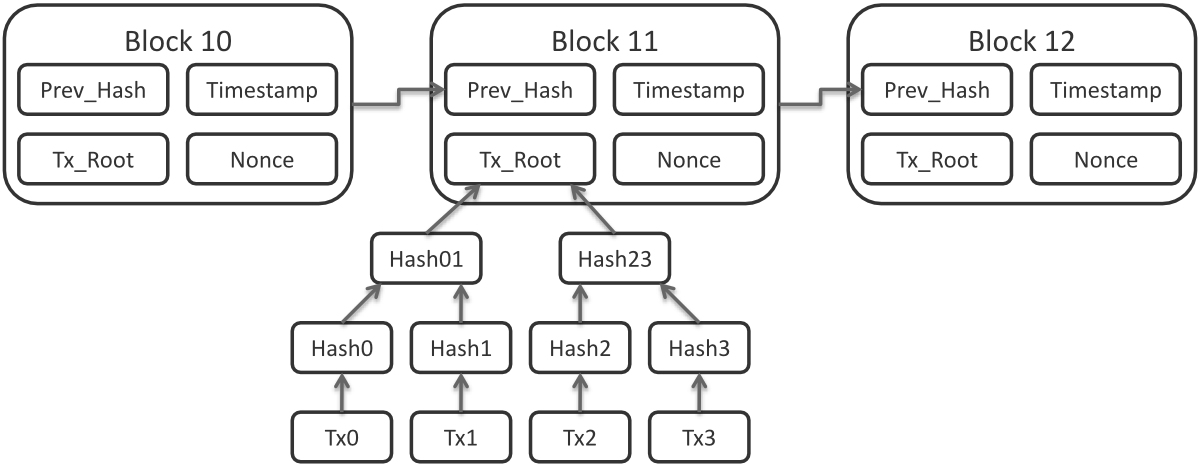
\includegraphics[width=0.9\textwidth]{./images-defense/bitcoin-blockchain.png}
\end{figure}

\end{frame}


\begin{frame}
\frametitle{Problems of Bitcoin}

Lack of scalability (up to 3.75 tx/s for 1MB per block)? Spam attacks?

\begin{figure}
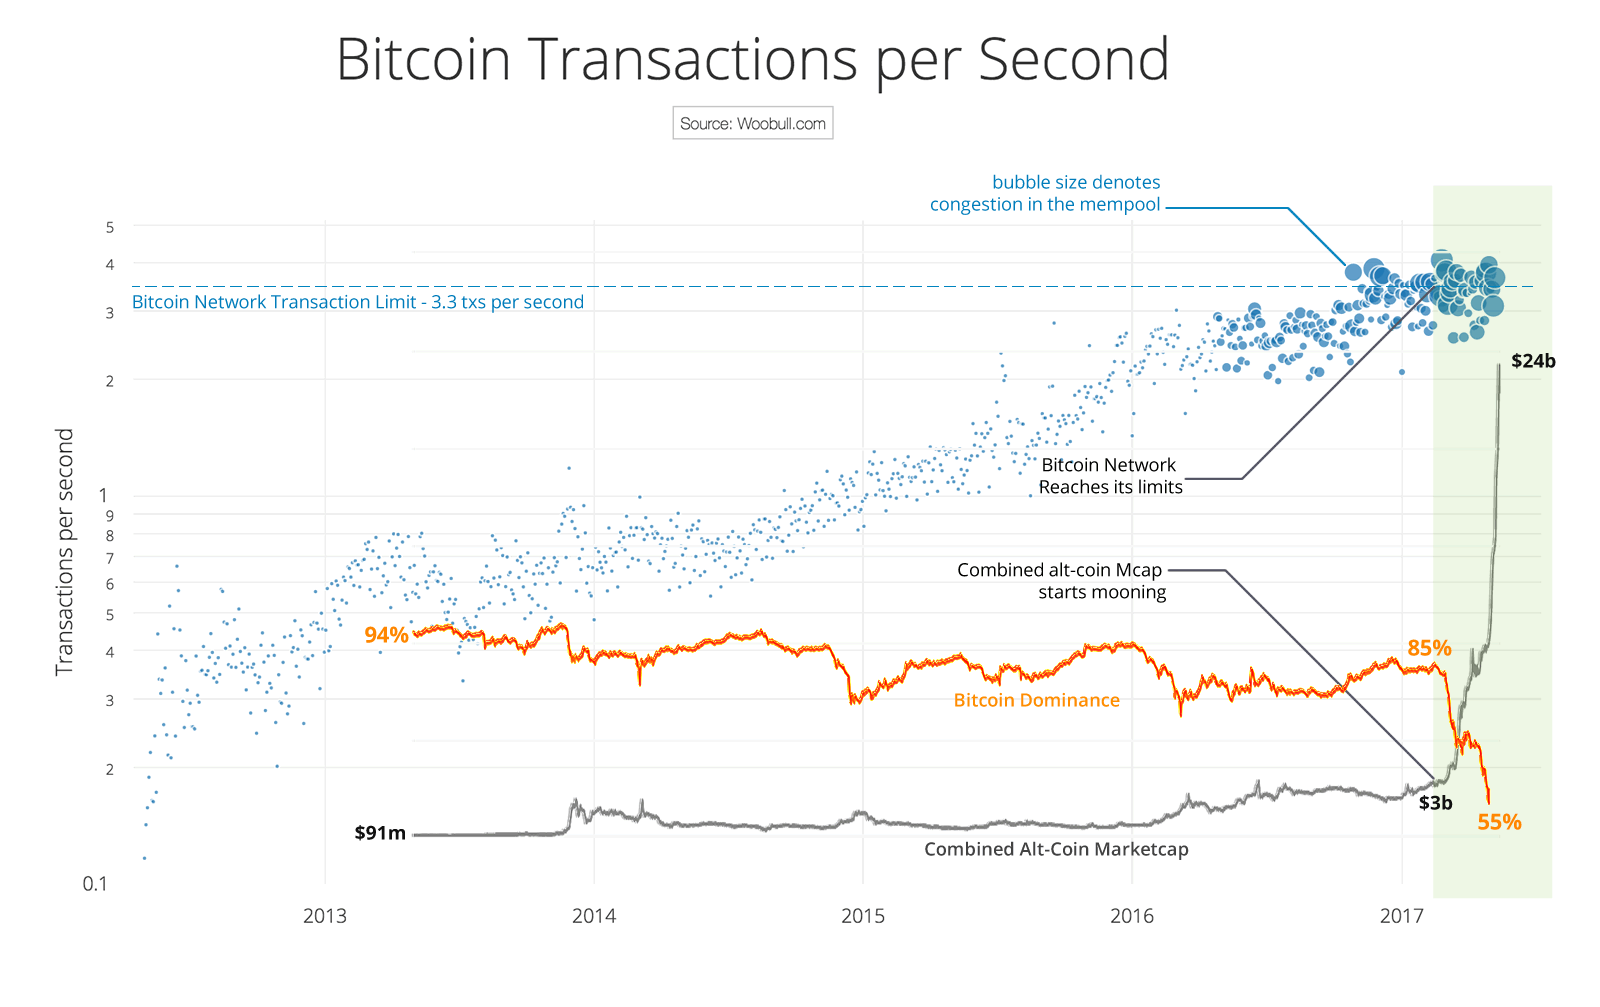
\includegraphics[width=0.8\textwidth]{./images-defense/bitcoin-congestion.png}
\end{figure}

\end{frame}


\begin{frame}
\frametitle{Iota \& Tangle}

\begin{figure}
\centering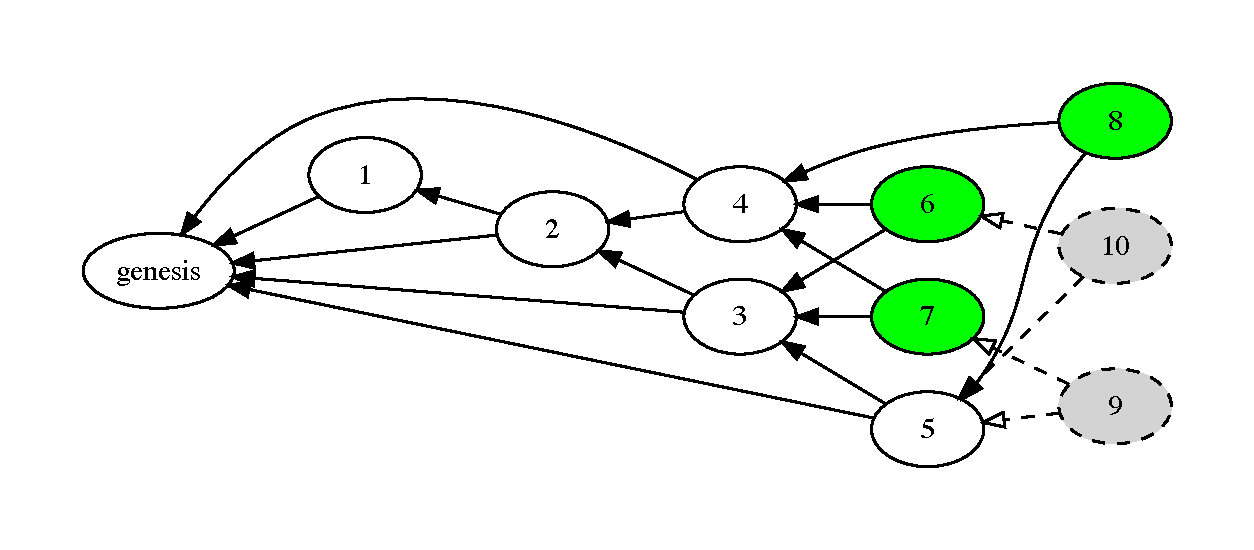
\includegraphics[width=0.8\textwidth]{./images01/fig-tangle-example.pdf}
\caption{White nodes represent transactions that have been confirmed at least once. Green circles represent unconfirmed transactions (tips). Gray and dashed nodes are the transactions currently solving the proof-of-work in order to be propagated.\label{fig-tangle-example}}
\end{figure}

\end{frame}


\begin{frame}
\frametitle{Problems of Iota}

\textbf{Iota is not safe in low load scenarios.} It must use a central coordinator to prevent attacks.

They plan to turn off the central coordinator, but \textbf{they do not know} what is the minimum number of transactions per seconds so that it is safe to do it.

\end{frame}


\begin{frame}
\frametitle{Hathor's architecture}

\begin{figure}
\centering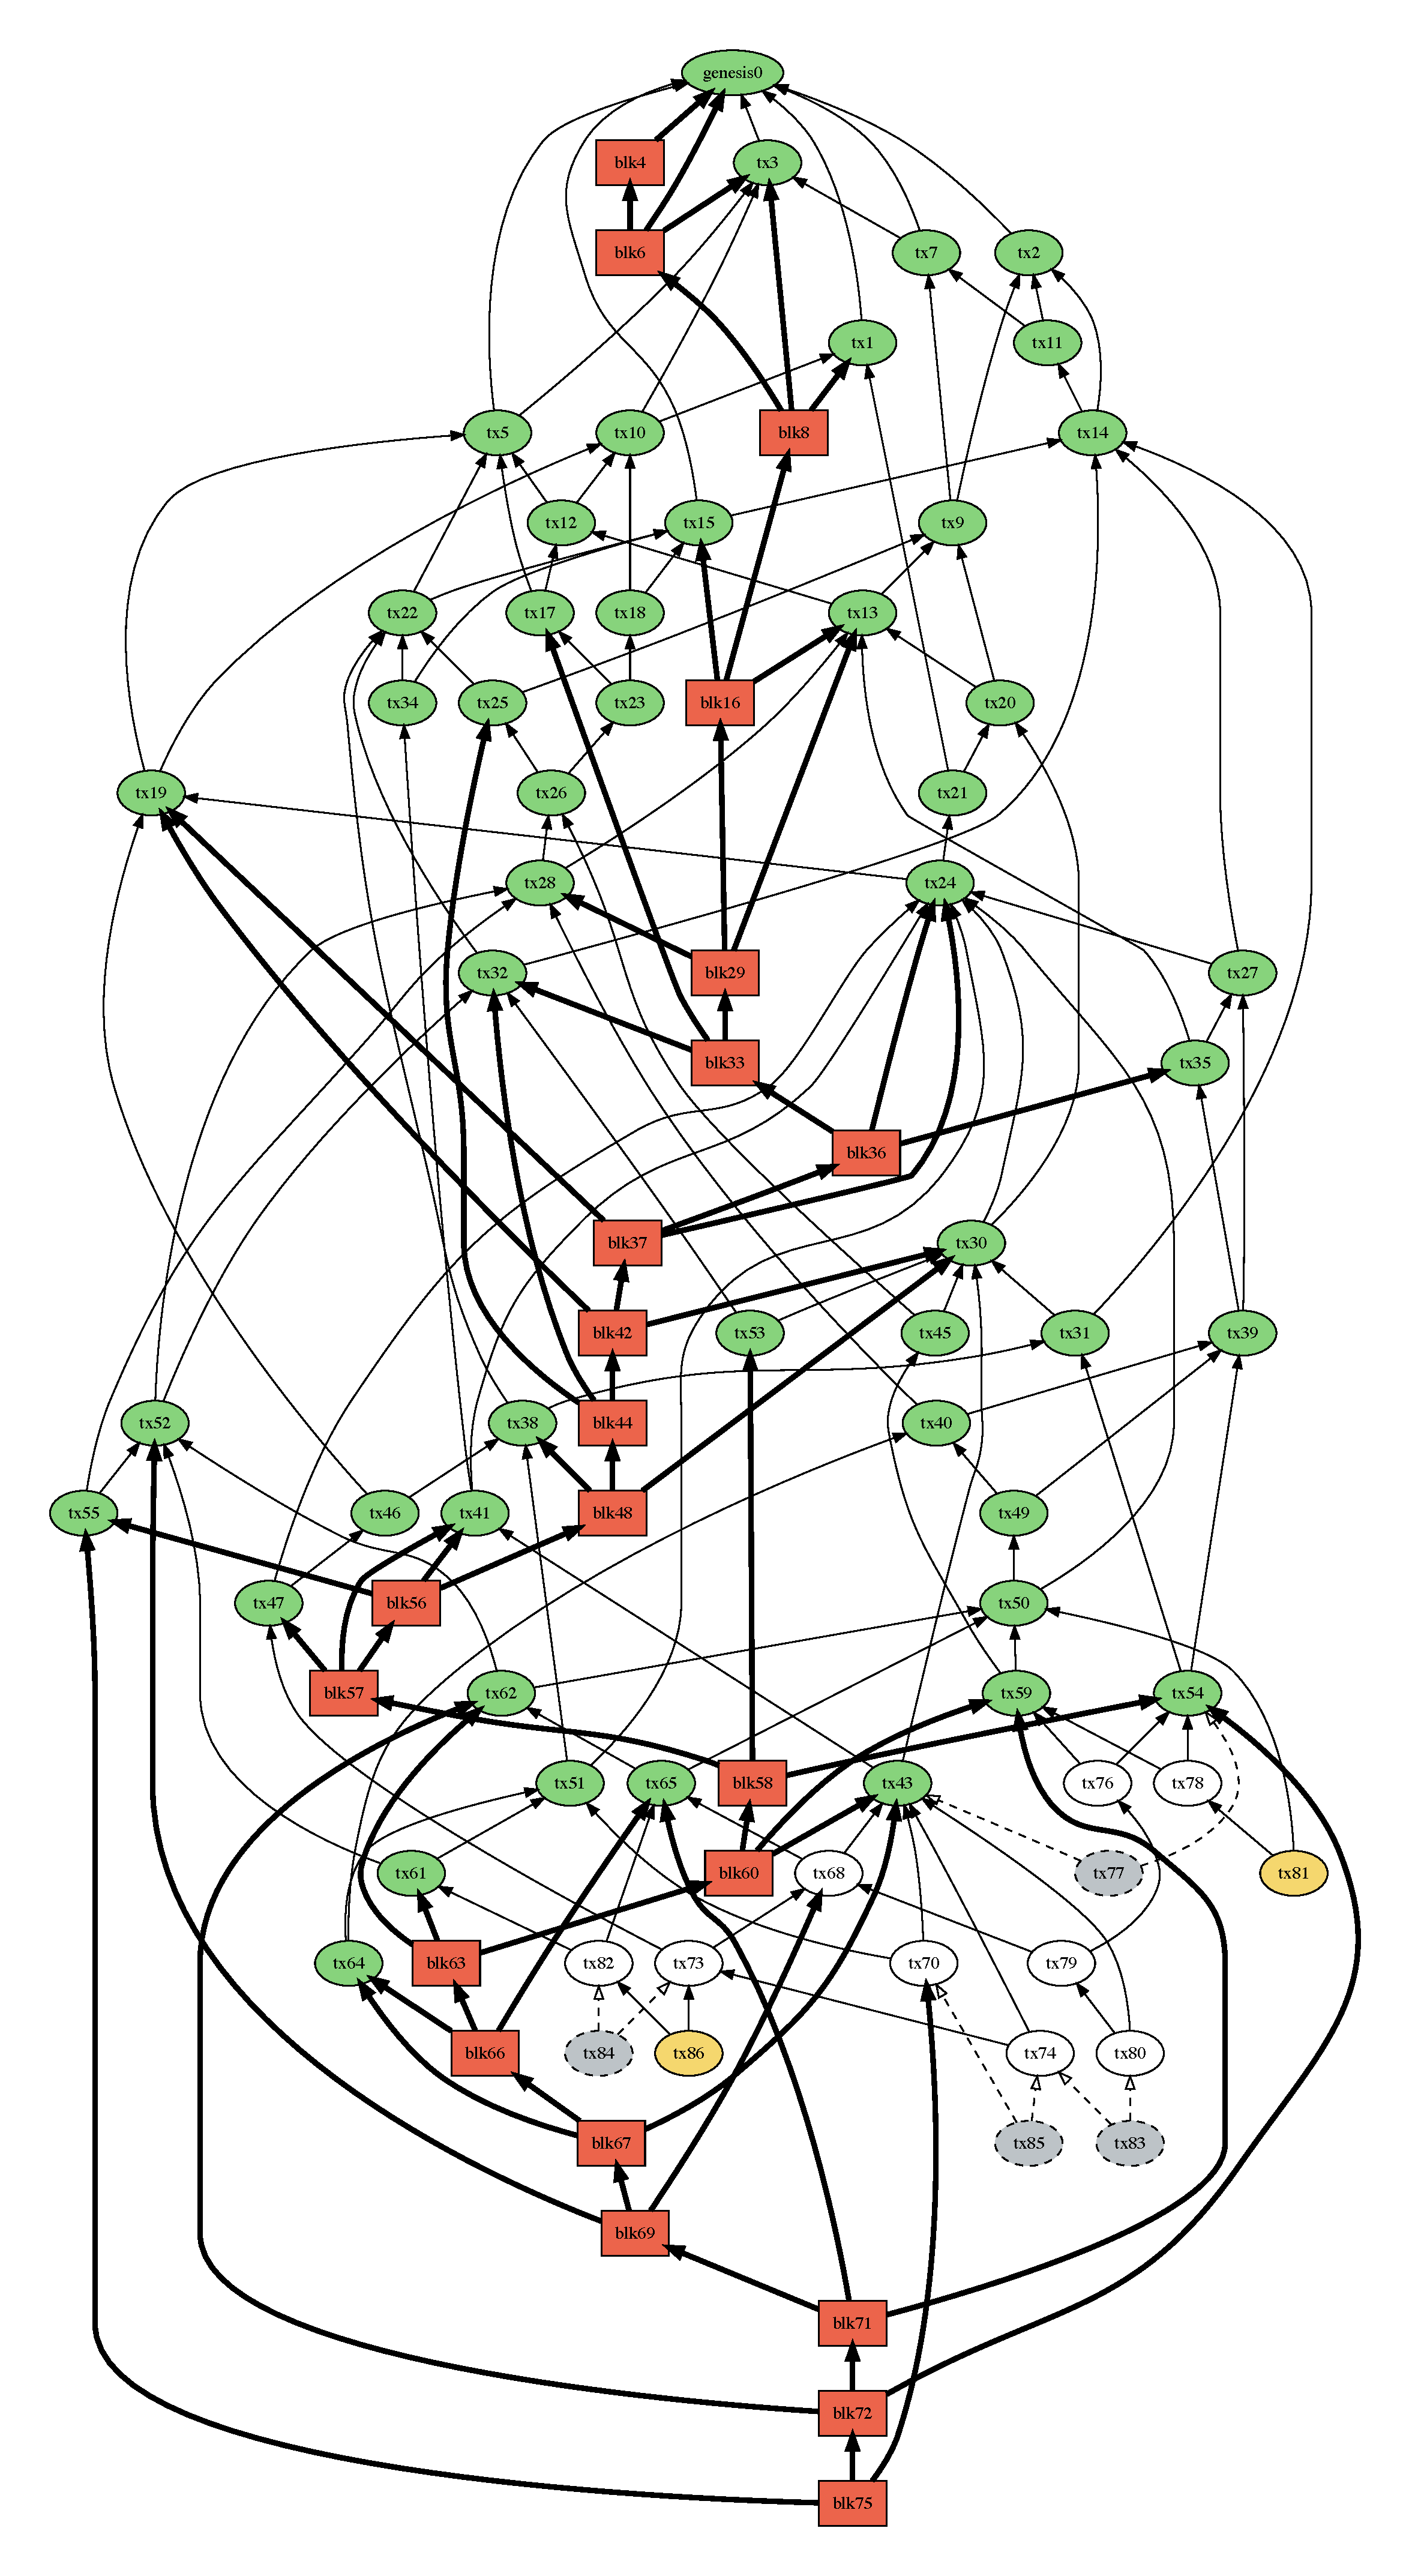
\includegraphics[width=0.45\textwidth]{./images01/sim/hathor-2.pdf}
\end{figure}

\end{frame}


\begin{frame}
\frametitle{Contributions}

The main contributions are:
\begin{enumerate}[i]
\item Mathematical analysis of Bitcoin
\item Proposal of Hathor, \emph{a novel architecture} which seems to work in both low and high load scenarios.
\item Analysis of Hathor
\end{enumerate}
\end{frame}


\begin{frame}
\frametitle{Mining the next block}

Each attempt to find a new block is equivalent to a random sample from a discrete uniform distribution in the interval $[0, 2^{256}-1]$. A new block is only found when the sample is less than a given number $A$.

The mining process is a sequence of failed attempts followed by a successful attempt. Let $X$ be the number of attempts until finding a new block. Then, $X$ follows a geometric distribution with probability $p = \frac{A}{2^{256}}$.

Let $H$ be the network hashpower, i.e., the number of attempts per second that the network is able to calculate. Thus, the time to find a new block (or the time between blocks) is $T = X/H$.

As $H$ changes over time, the given number $A$ is adjusted so that the network would find a block every $\eta$ seconds, which leads to $P(T \le t) = 1 - \left(1 - \frac{1}{\eta H} \right)^{tH}$.
\end{frame}


\begin{frame}
\frametitle{Mining the next block (2)}

\begin{theorem}
    For $H$ large enough, the time between blocks may be approximated by an exponential distribution, i.e., $P(T \le t) = 1 - e^{t/\eta}$.
\end{theorem}

\begin{theorem}
	The maximum absolute error when approximating the time between blocks by an exponential distribution is $e / H$.
\end{theorem}

So, for a maximum absolute error of $0.01 \% = 10^{-4}$, the network hashpower $H$ must be at least 26 kH/s.

For comparison, Bitcoin's hashpower is around 35,000,000 TH/s = 35,000,000,000,000,000 kH/s = $35 \cdot 10^{18} H/s$. In this case, the maximum absolute error is $7.7 \cdot 10^{-20} = 0.0000000000000000000776$.

\end{frame}


\begin{frame}
\frametitle{Bitcoin's hashpower history}
\begin{figure}
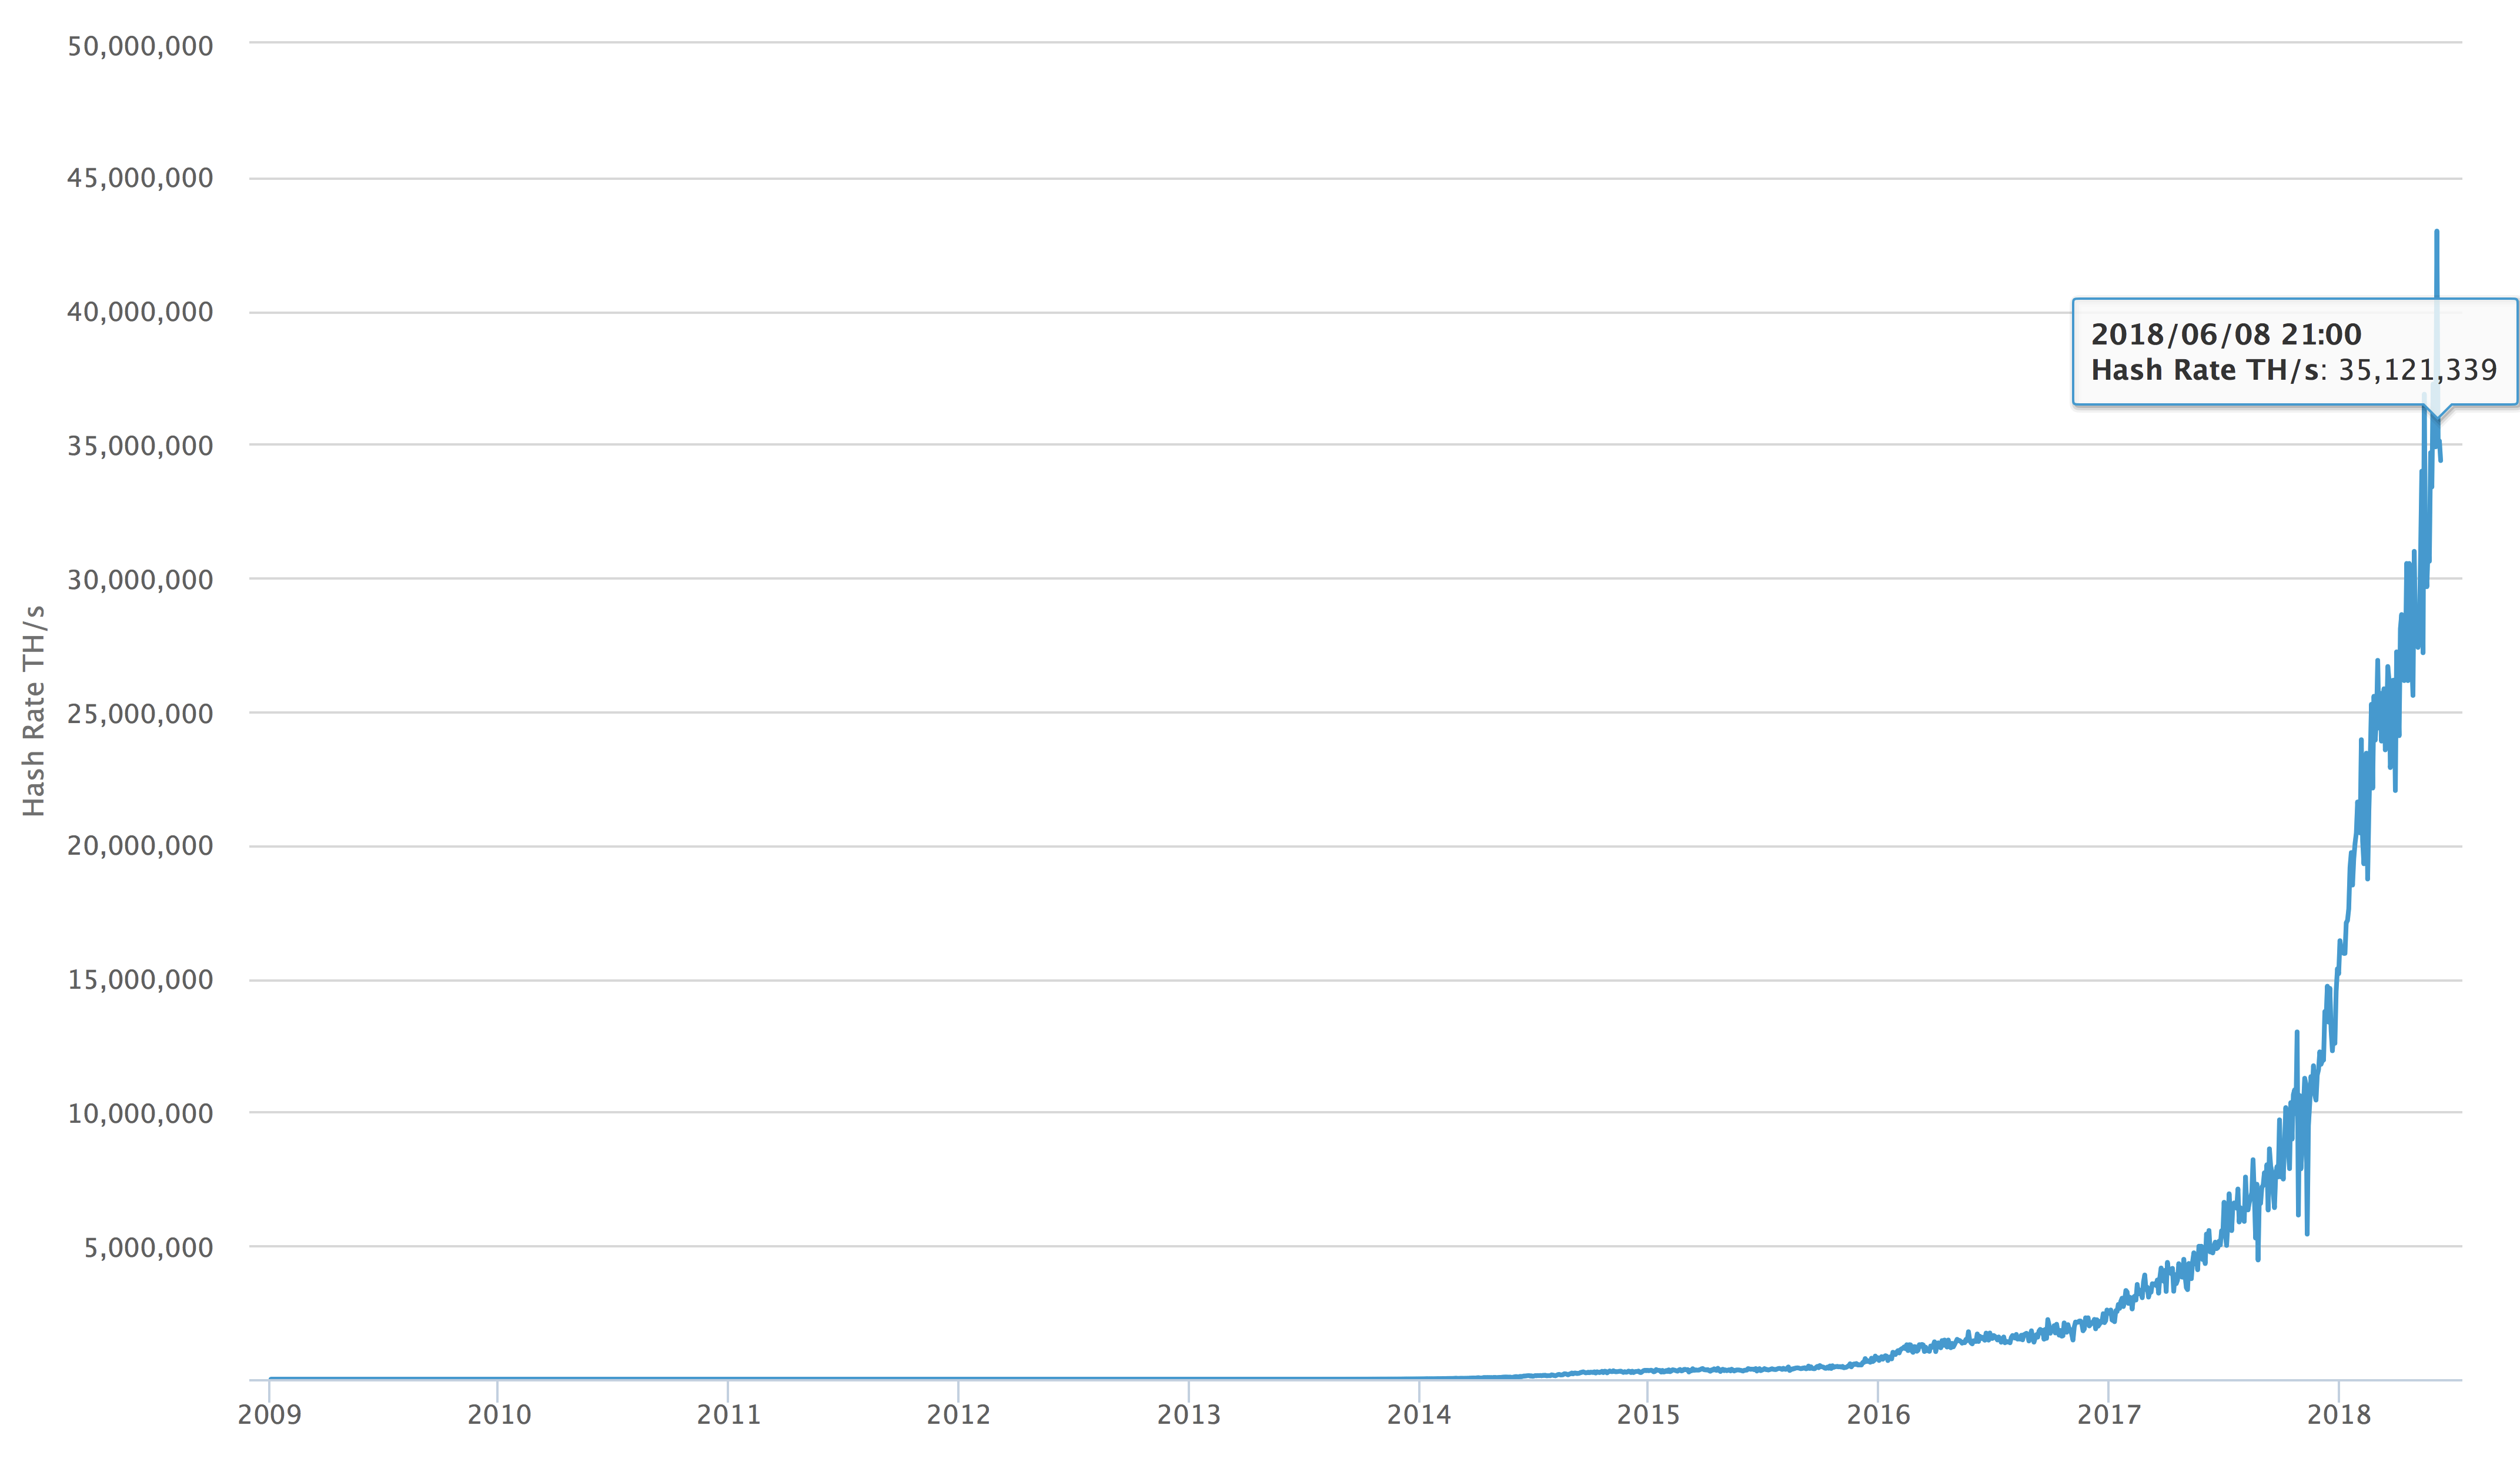
\includegraphics[width=\textwidth]{./images-defense/bitcoin-H-history.png}
\end{figure}
\end{frame}


\begin{frame}
\frametitle{Mining consecutive blocks}

Let $Y_n = \sum_{i=1}^n T_i$ be the total time to find $n$ consecutive blocks. From probability literature, $Y_n$ follows an Erlang distribution.

\begin{figure}
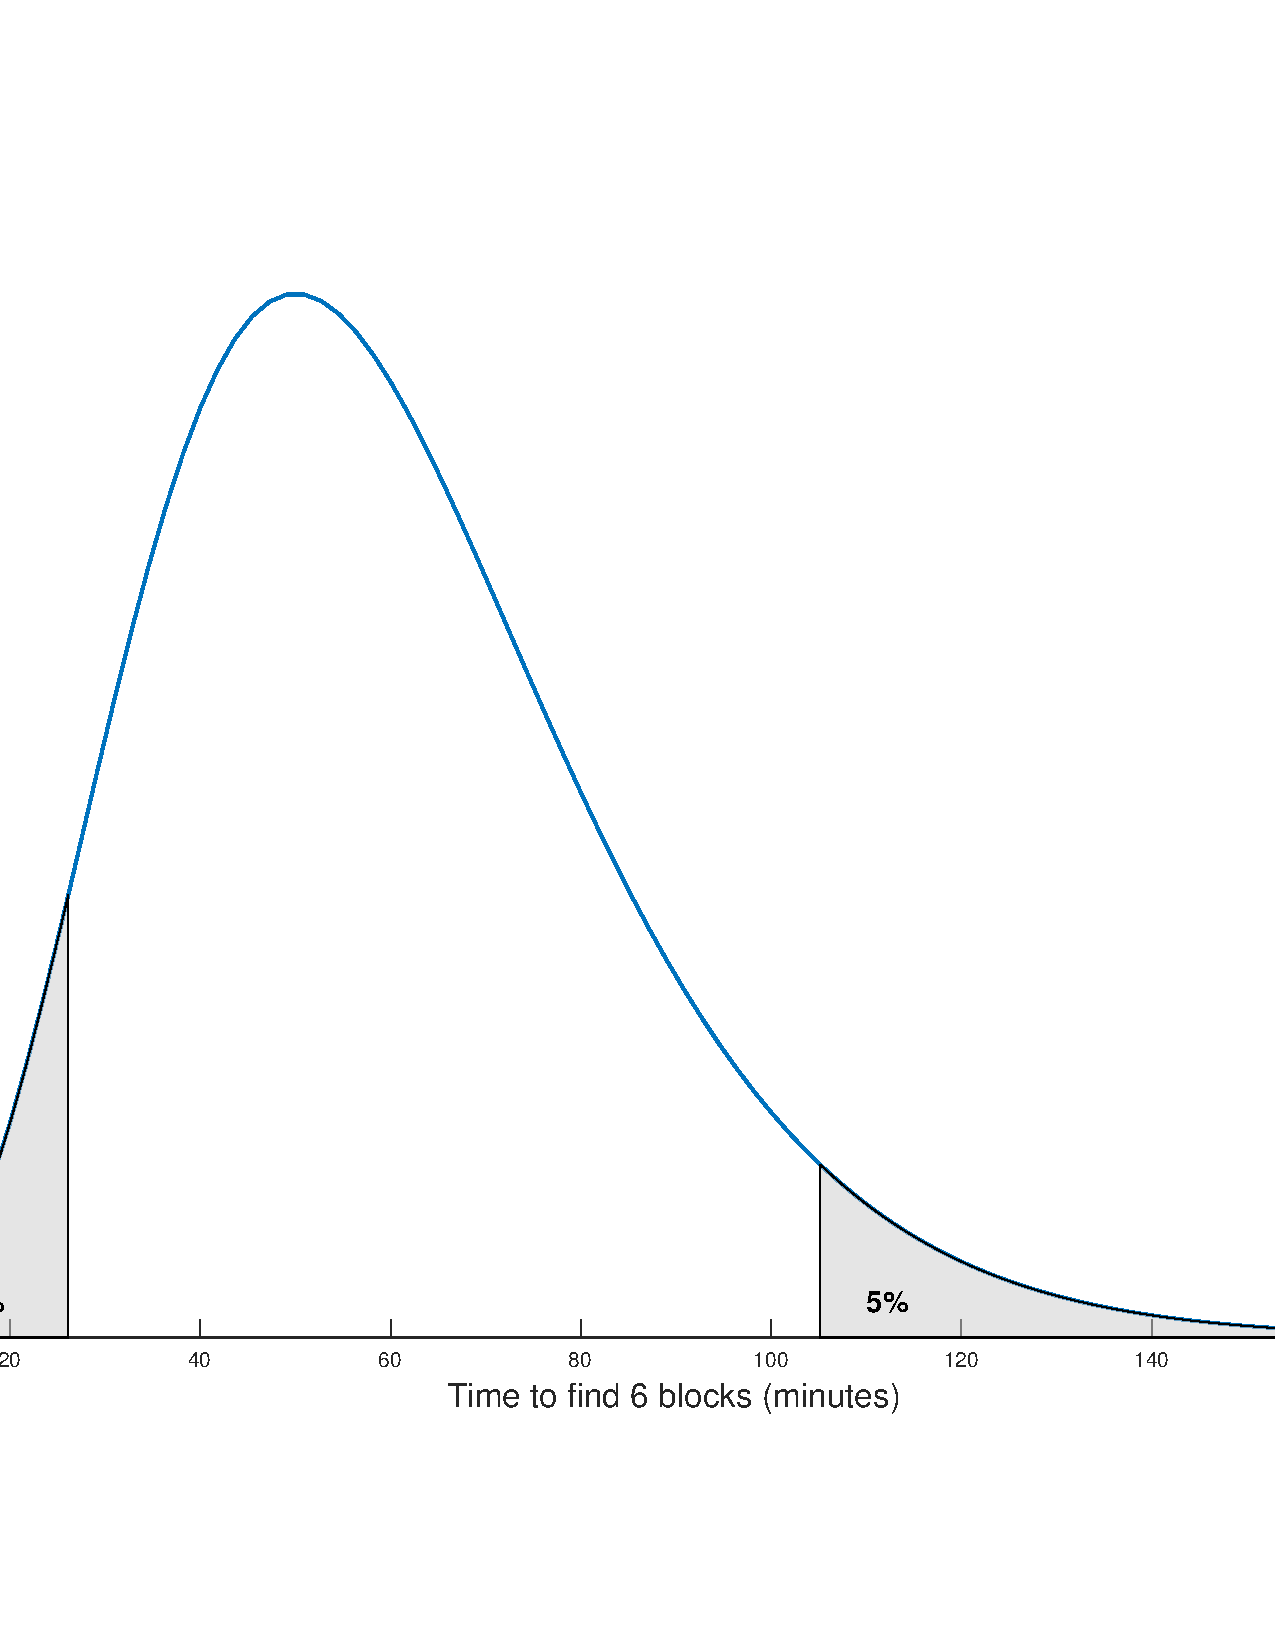
\includegraphics[width=0.7\textwidth]{./images01/time-6-blocks.pdf}
\caption{PDF of $Y_6$, i.e., probability of finding 6 consecutive blocks.}
\end{figure}

\end{frame}


\begin{frame}
\frametitle{The double-spending attack}

In the double spending attack, \textbf{the attacker's send some funds to the victim}, let's say a merchant.

They wait for $k$ confirmations of the transaction, and \textbf{the victim delivers the good or the service to the attacker}.

Then, the attacker mine enough blocks \textbf{with a conflicting transaction}, double spending the funds which was sent to the victim.

If the attacker is successful, the original transaction will be \textit{erased} and \textbf{the victim will be left with no funds at all}.

\end{frame}


\begin{frame}
\frametitle{Attack in the Bitcoin network}

\begin{theorem}
	Let $\beta$ be the percentage of the hashpower controlled by the attacker, and $\gamma$ the percentage of the hashpower without the attacker. Let $p = \frac{\gamma}{\beta + \gamma}$. Then,
$$
\mathbf{P}(\text{successful attack}) =
\begin{cases}
	1 - \sum_{s=0}^{k-1} \binom{k+s-1}{s} \left( (1-p)^s p^k - (1-p)^k p^s \right) \text{, $p \geq 0.5$} \\
	1 \text{, $\gamma < \beta$}.\\
\end{cases}
$$
\end{theorem}

For $k=6$, $p=0.9$, $\mathbf{P}(\text{successful attack}) = 0.0005914121600000266$.

For $k=6$, $p=0.7$, $\mathbf{P}(\text{successful attack}) = 0.15644958192000014$.

\end{frame}


\begin{frame}
\frametitle{Attack in the Bitcoin network}
\begin{figure}
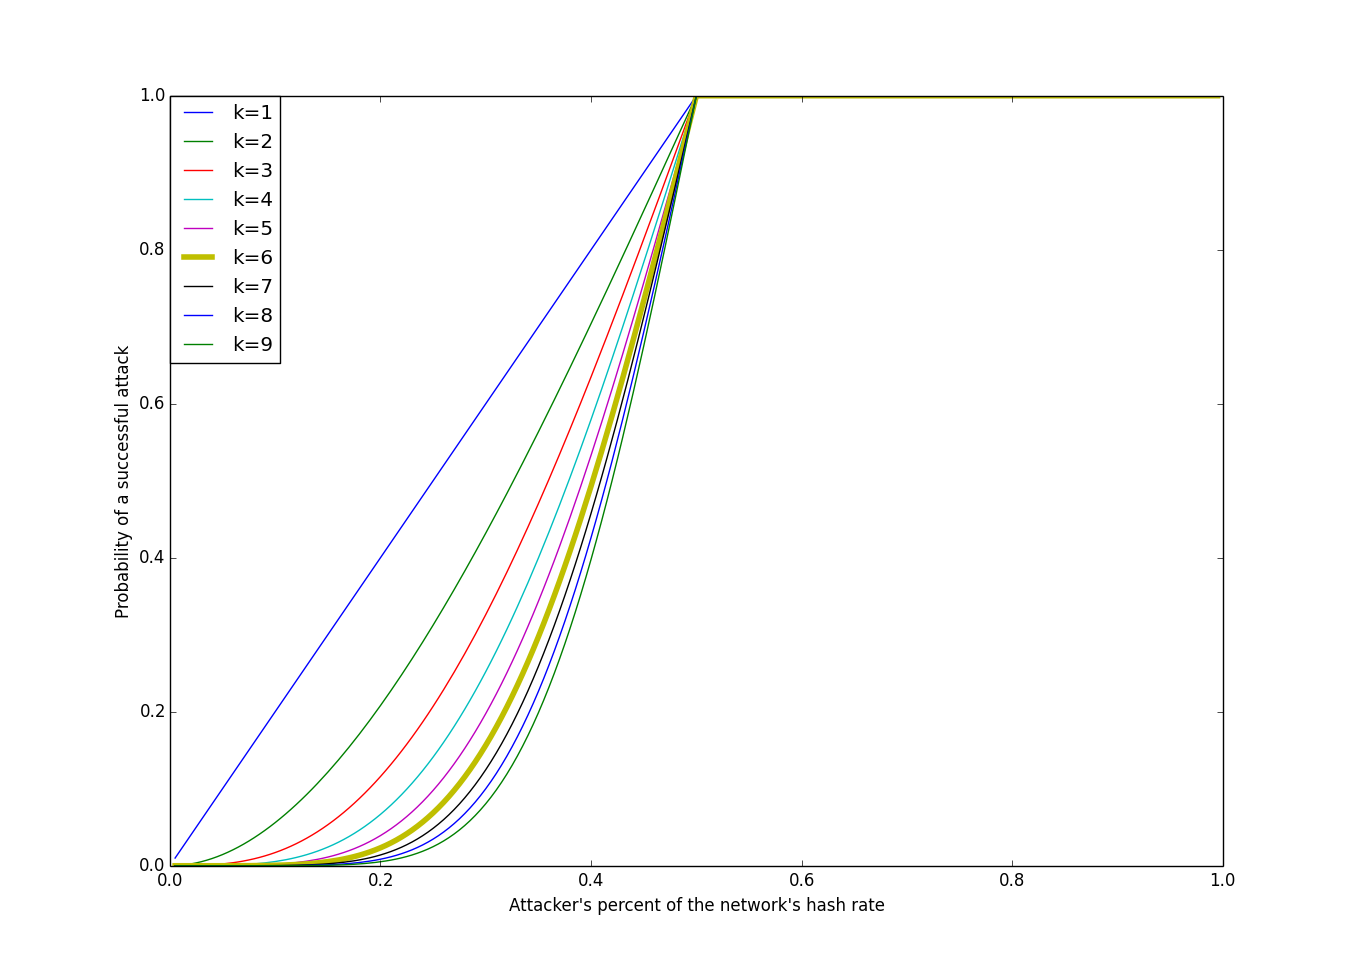
\includegraphics[width=0.75\textwidth]{./images01/fig-bitcoin-attack.png}
\caption{Probability of a successful attack according to the network's hash rate of the attacker ($\beta$).}
\end{figure}
\end{frame}


\begin{frame}
\frametitle{Analysis of Hathor}

\begin{figure}
\centering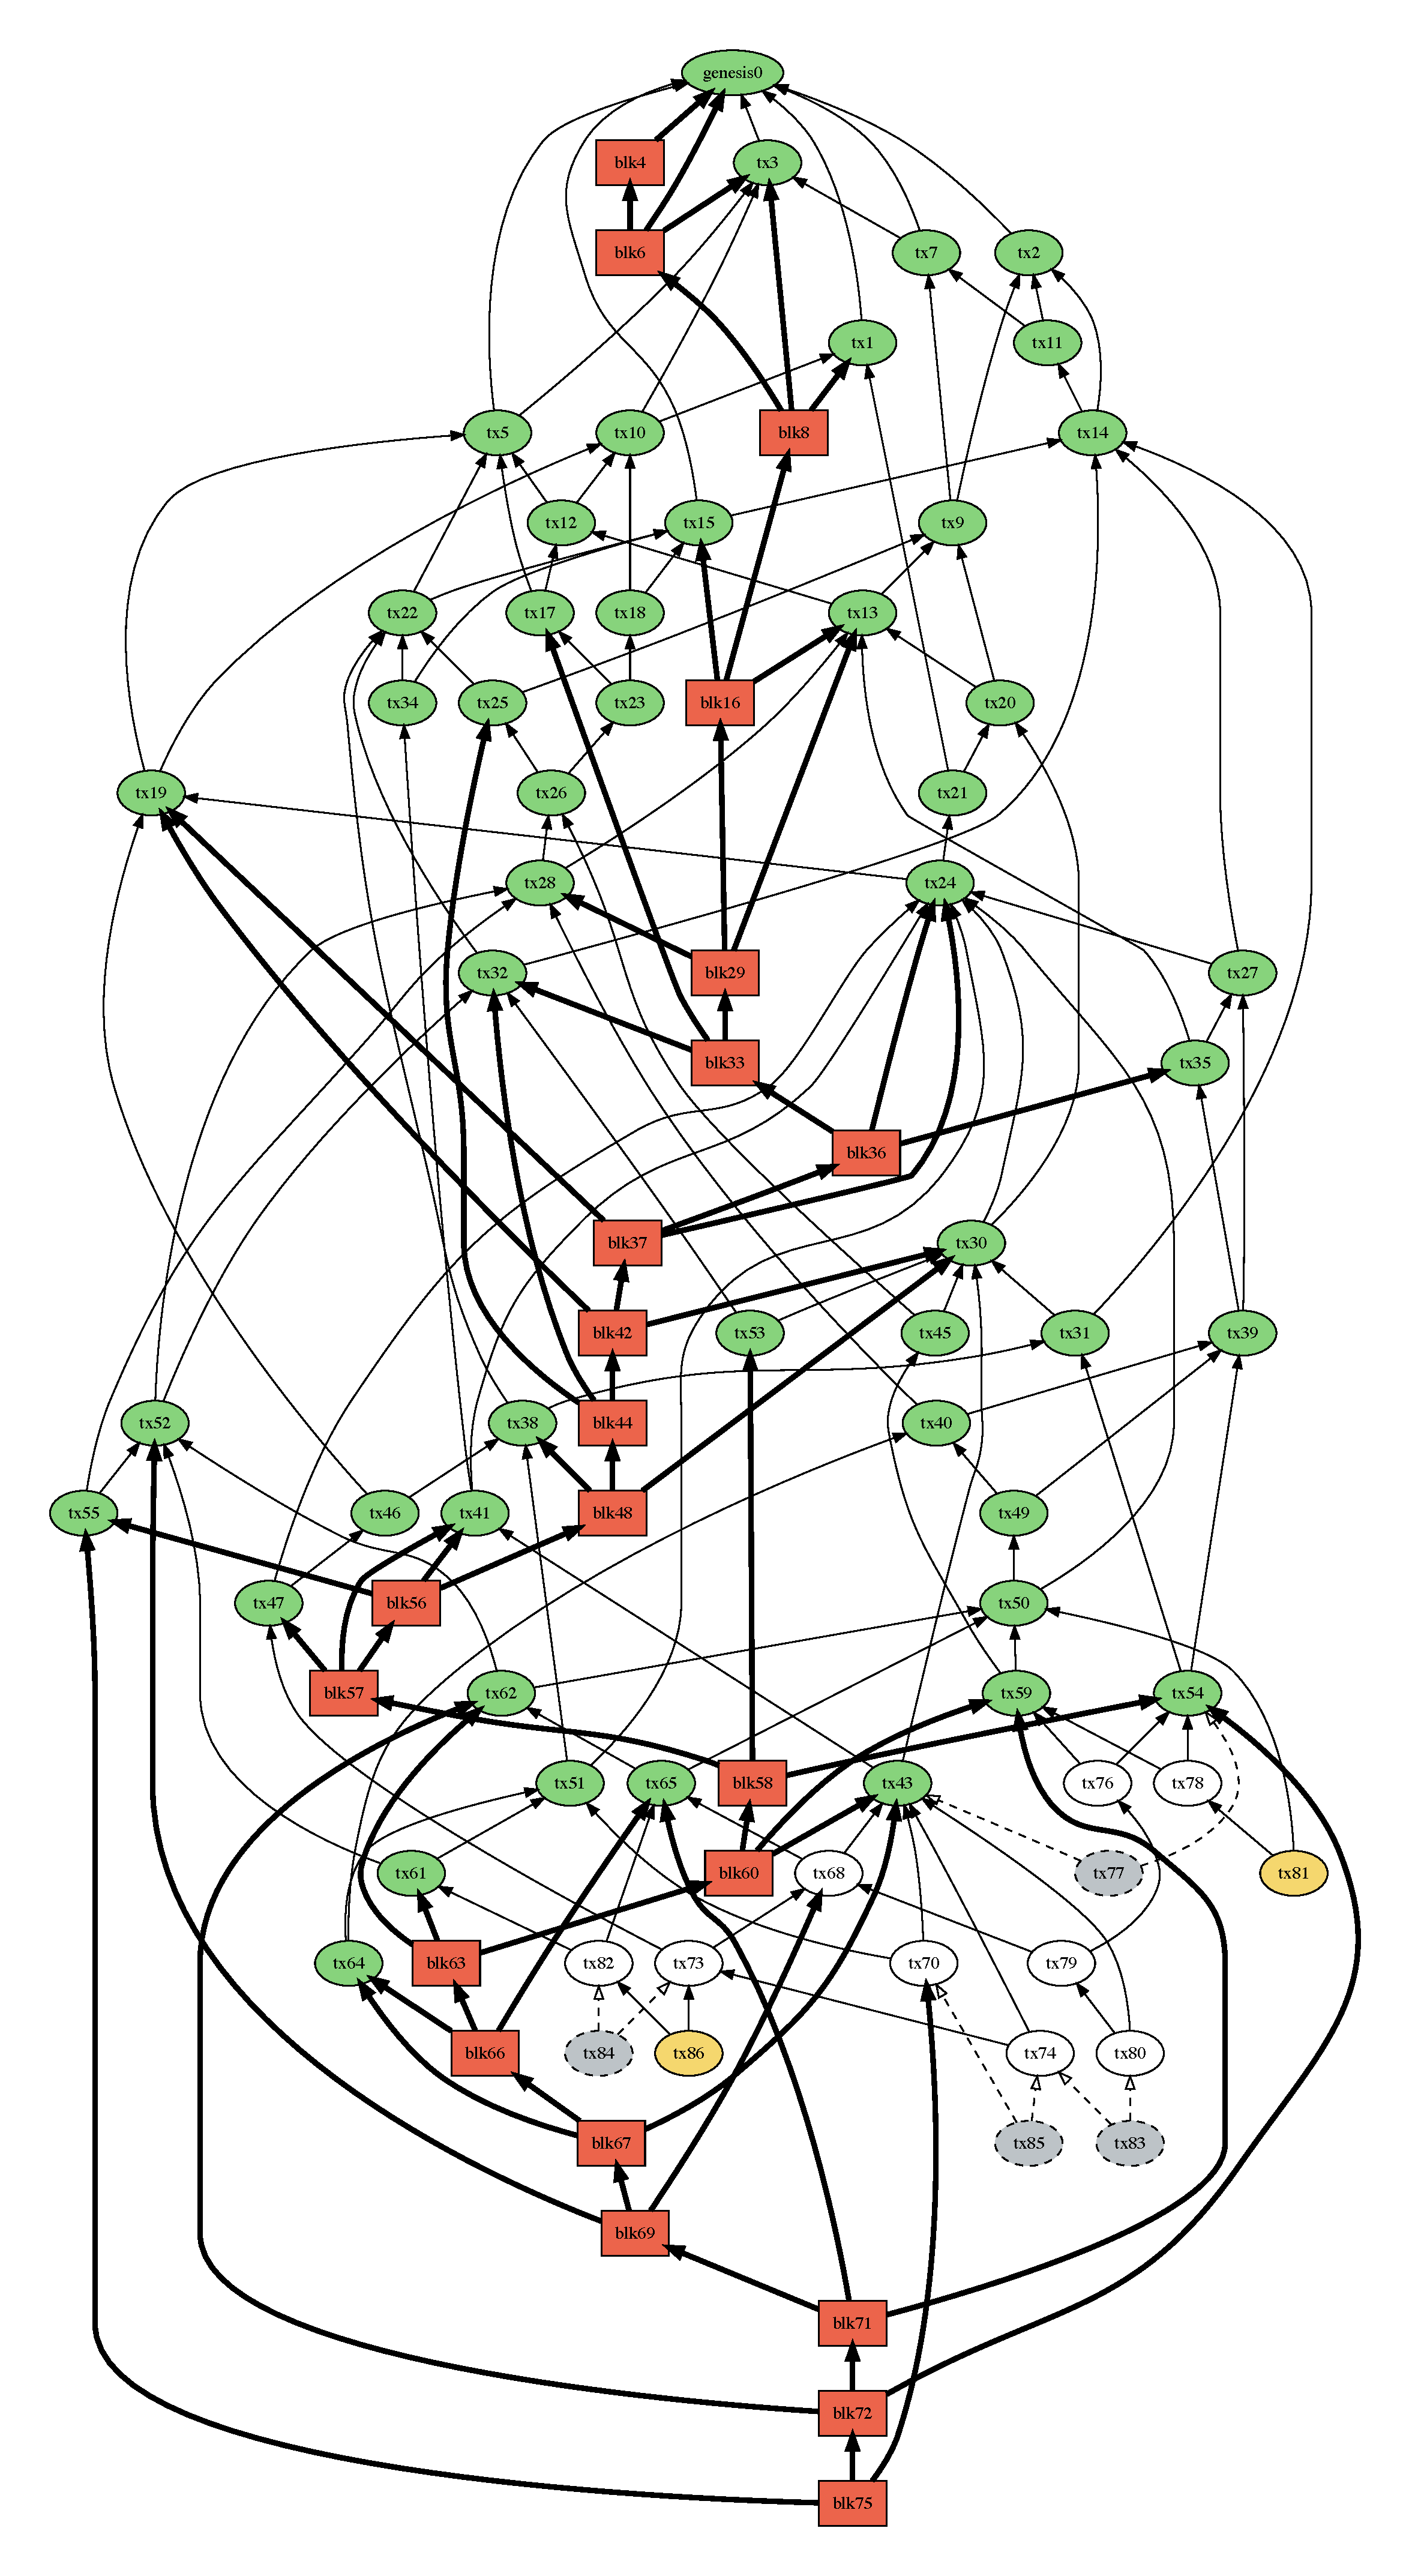
\includegraphics[width=0.45\textwidth]{./images01/sim/hathor-2.pdf}
\end{figure}

\end{frame}


\begin{frame}
\frametitle{Analysis of Hathor: Boundary cases}

\begin{figure}
\centering
\subfloat[No miners]{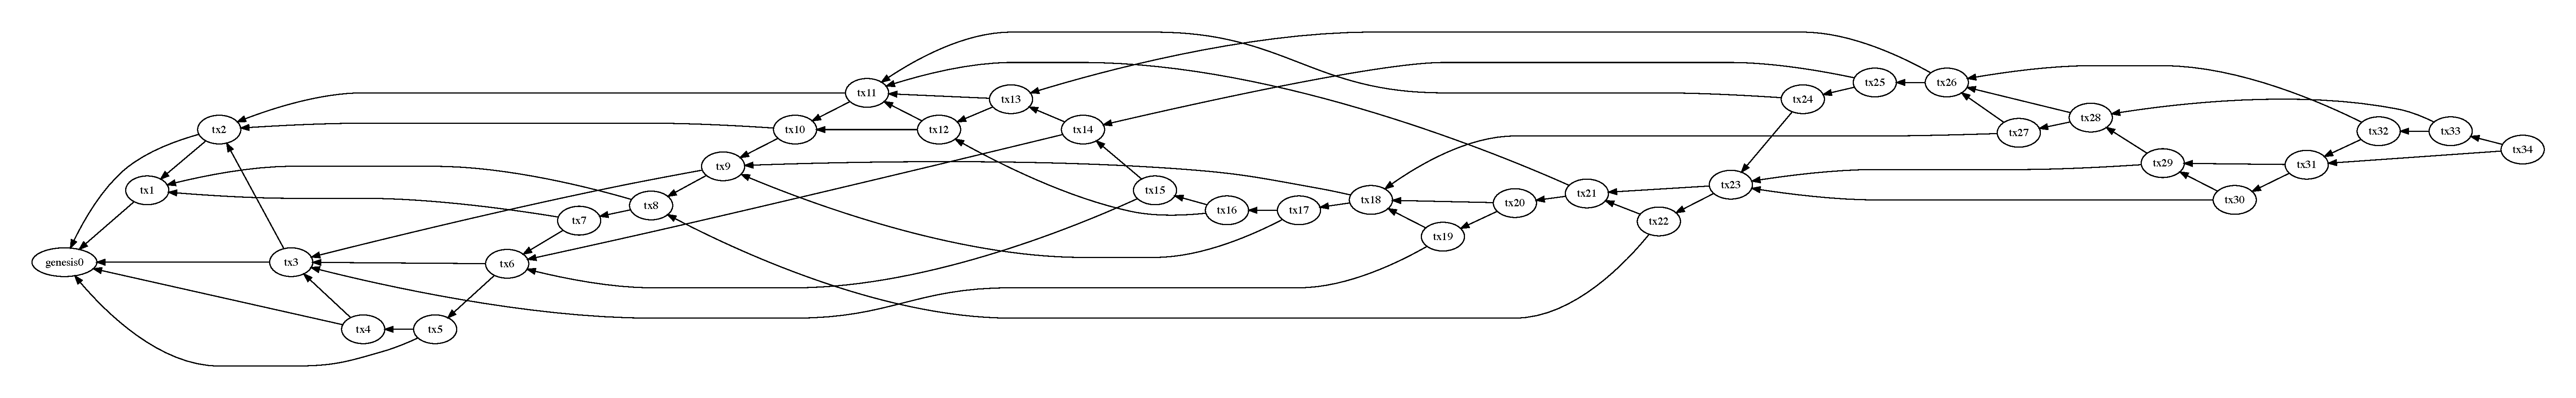
\includegraphics[width=0.5\textwidth]{./images01/sim/no_miners.pdf}}
\subfloat[No transactions]{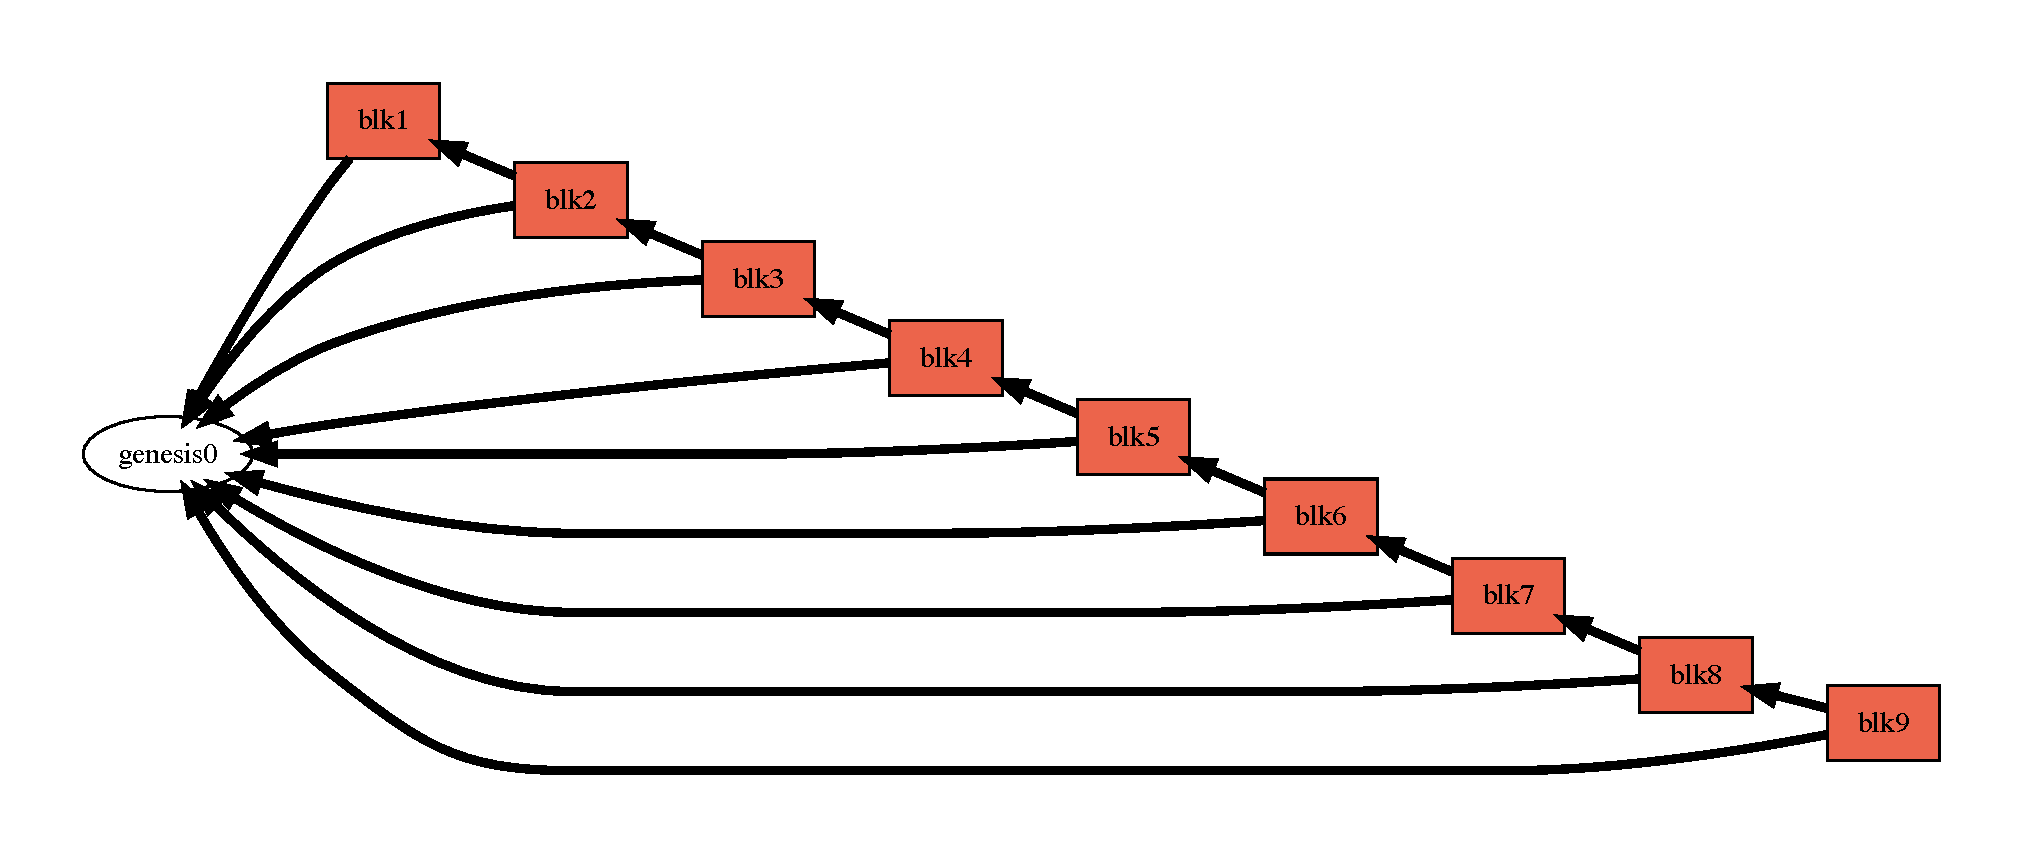
\includegraphics[width=0.5\textwidth]{./images01/sim/only_miners.pdf}}
\caption{Visualization of a Hathor's graph in two particular cases: (a) no miners, (b) no transactions.}
\end{figure}

\end{frame}


\begin{frame}
\frametitle{Analysis of Hathor: Confirmation time}
\begin{figure}
\centering
\subfloat[Low load]{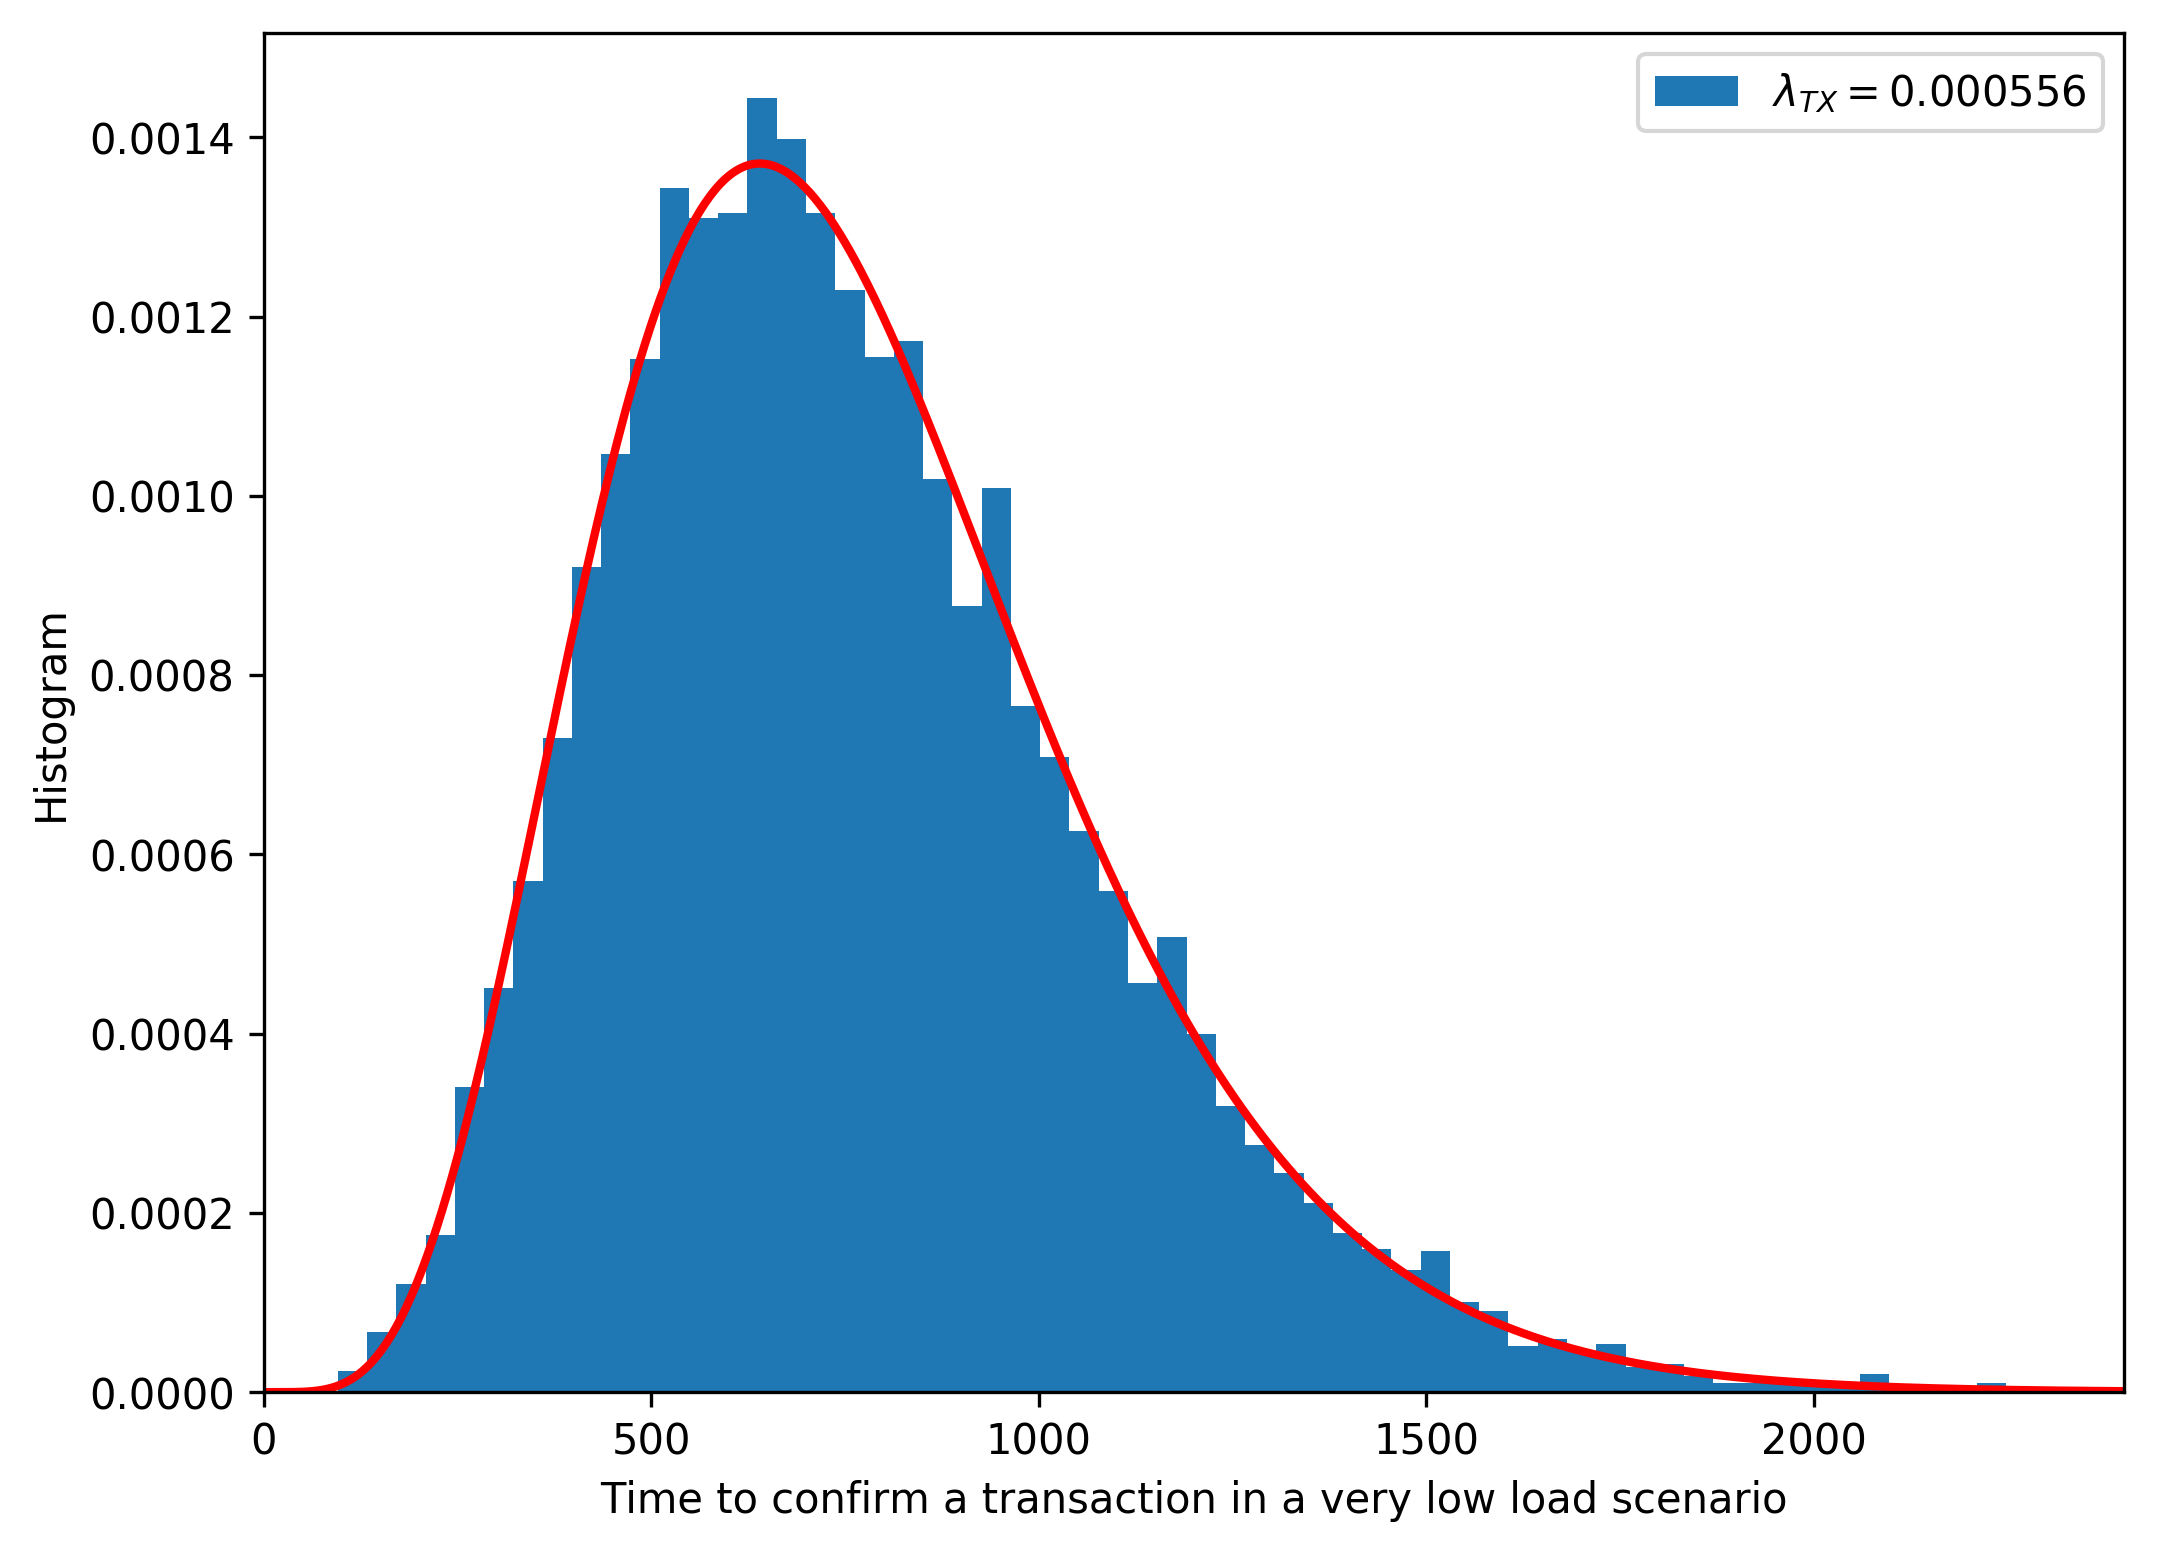
\includegraphics[width=0.5\textwidth]{./images01/sim/tct-low-load.png}}
\subfloat[Mid load]{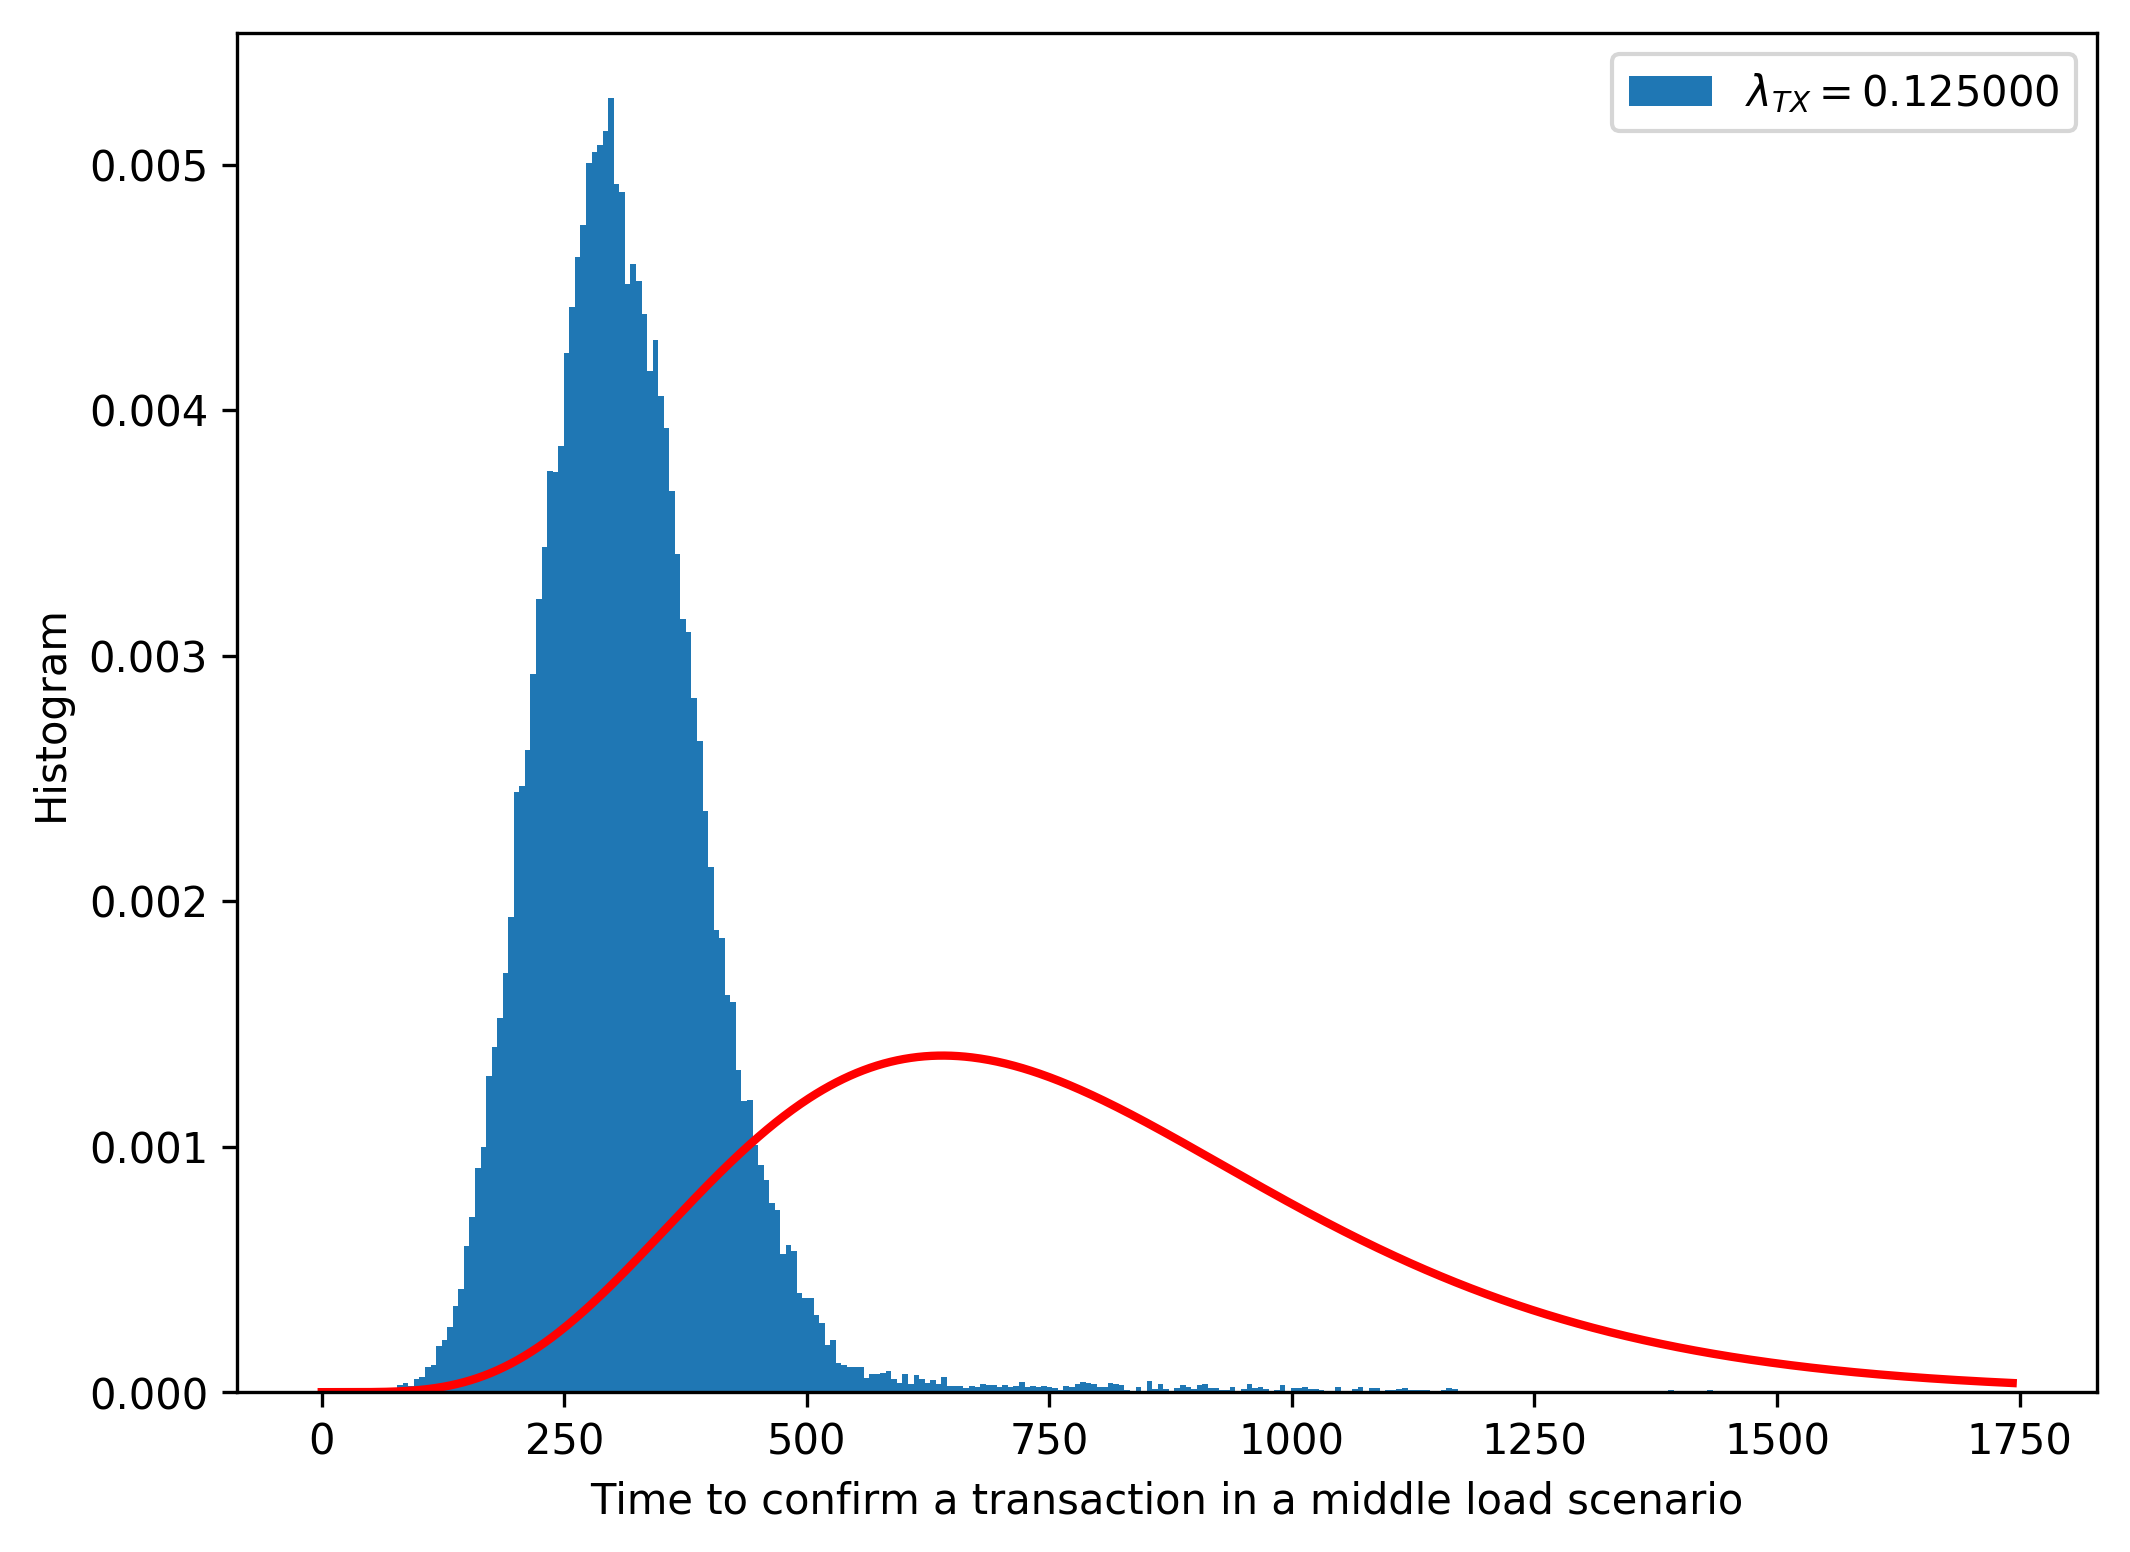
\includegraphics[width=0.5\textwidth]{./images01/sim/tct-mid-load.png}}

\caption{Confirmation time in two scenarios: (a) low load, (b) mid load. The red curve is the distribuion of the time to find six blocks in Bitcoin (which follows an Erlang distribution).}
\end{figure}
\end{frame}


\begin{frame}
\frametitle{Analysis of Hathor: Confirmation time (2)}
\begin{figure}
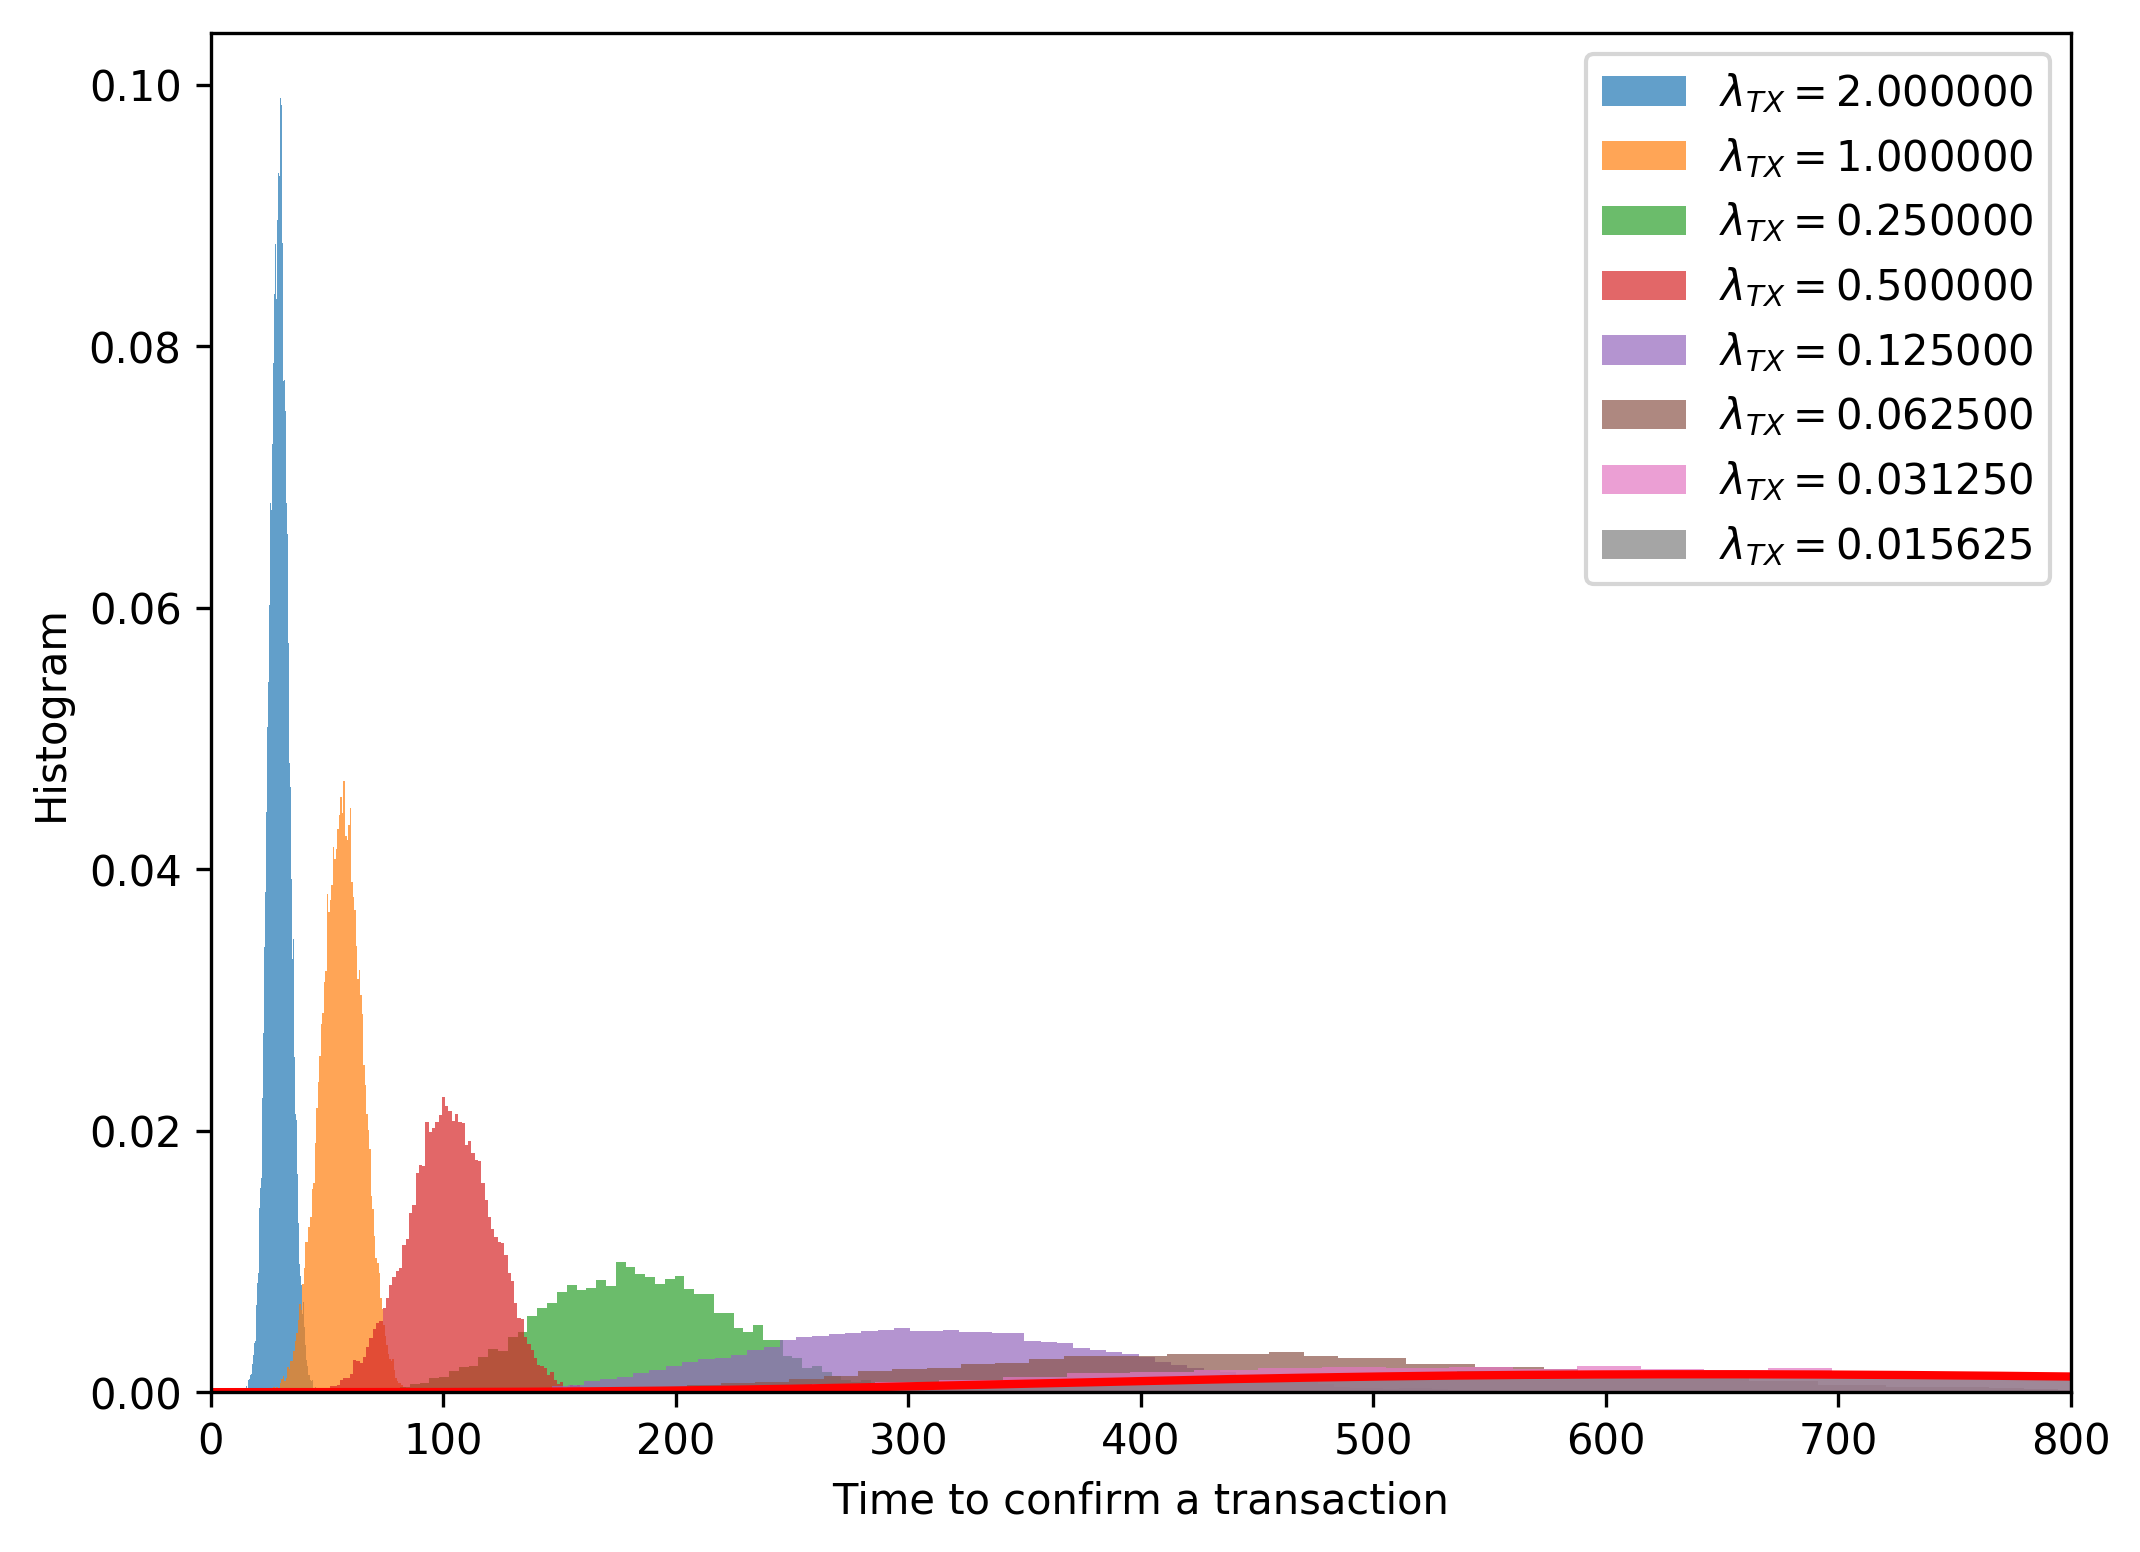
\includegraphics[width=0.75\textwidth]{./images01/sim/tct-many-loads-2.png}

\caption{Confirmation time in many scenarios, moving from a low load ($\lambda_\text{TX} = 0.015625$) to a high load ($\lambda_\text{TX} = 2$). \label{fig:hathor-tct-many}}
\end{figure}
\end{frame}


\begin{frame}
\frametitle{Analysis of Hathor: Load changing over time}
\begin{figure}
\centering
\includegraphics[width=\textwidth]{./images01/new/many-loadings.pdf}
\caption{DAG visualization when the loading is changed over time.}
\end{figure}
\end{frame}


\begin{frame}
\frametitle{Analysis of Hathor: Number of unconfirmed transactions}
\begin{figure}
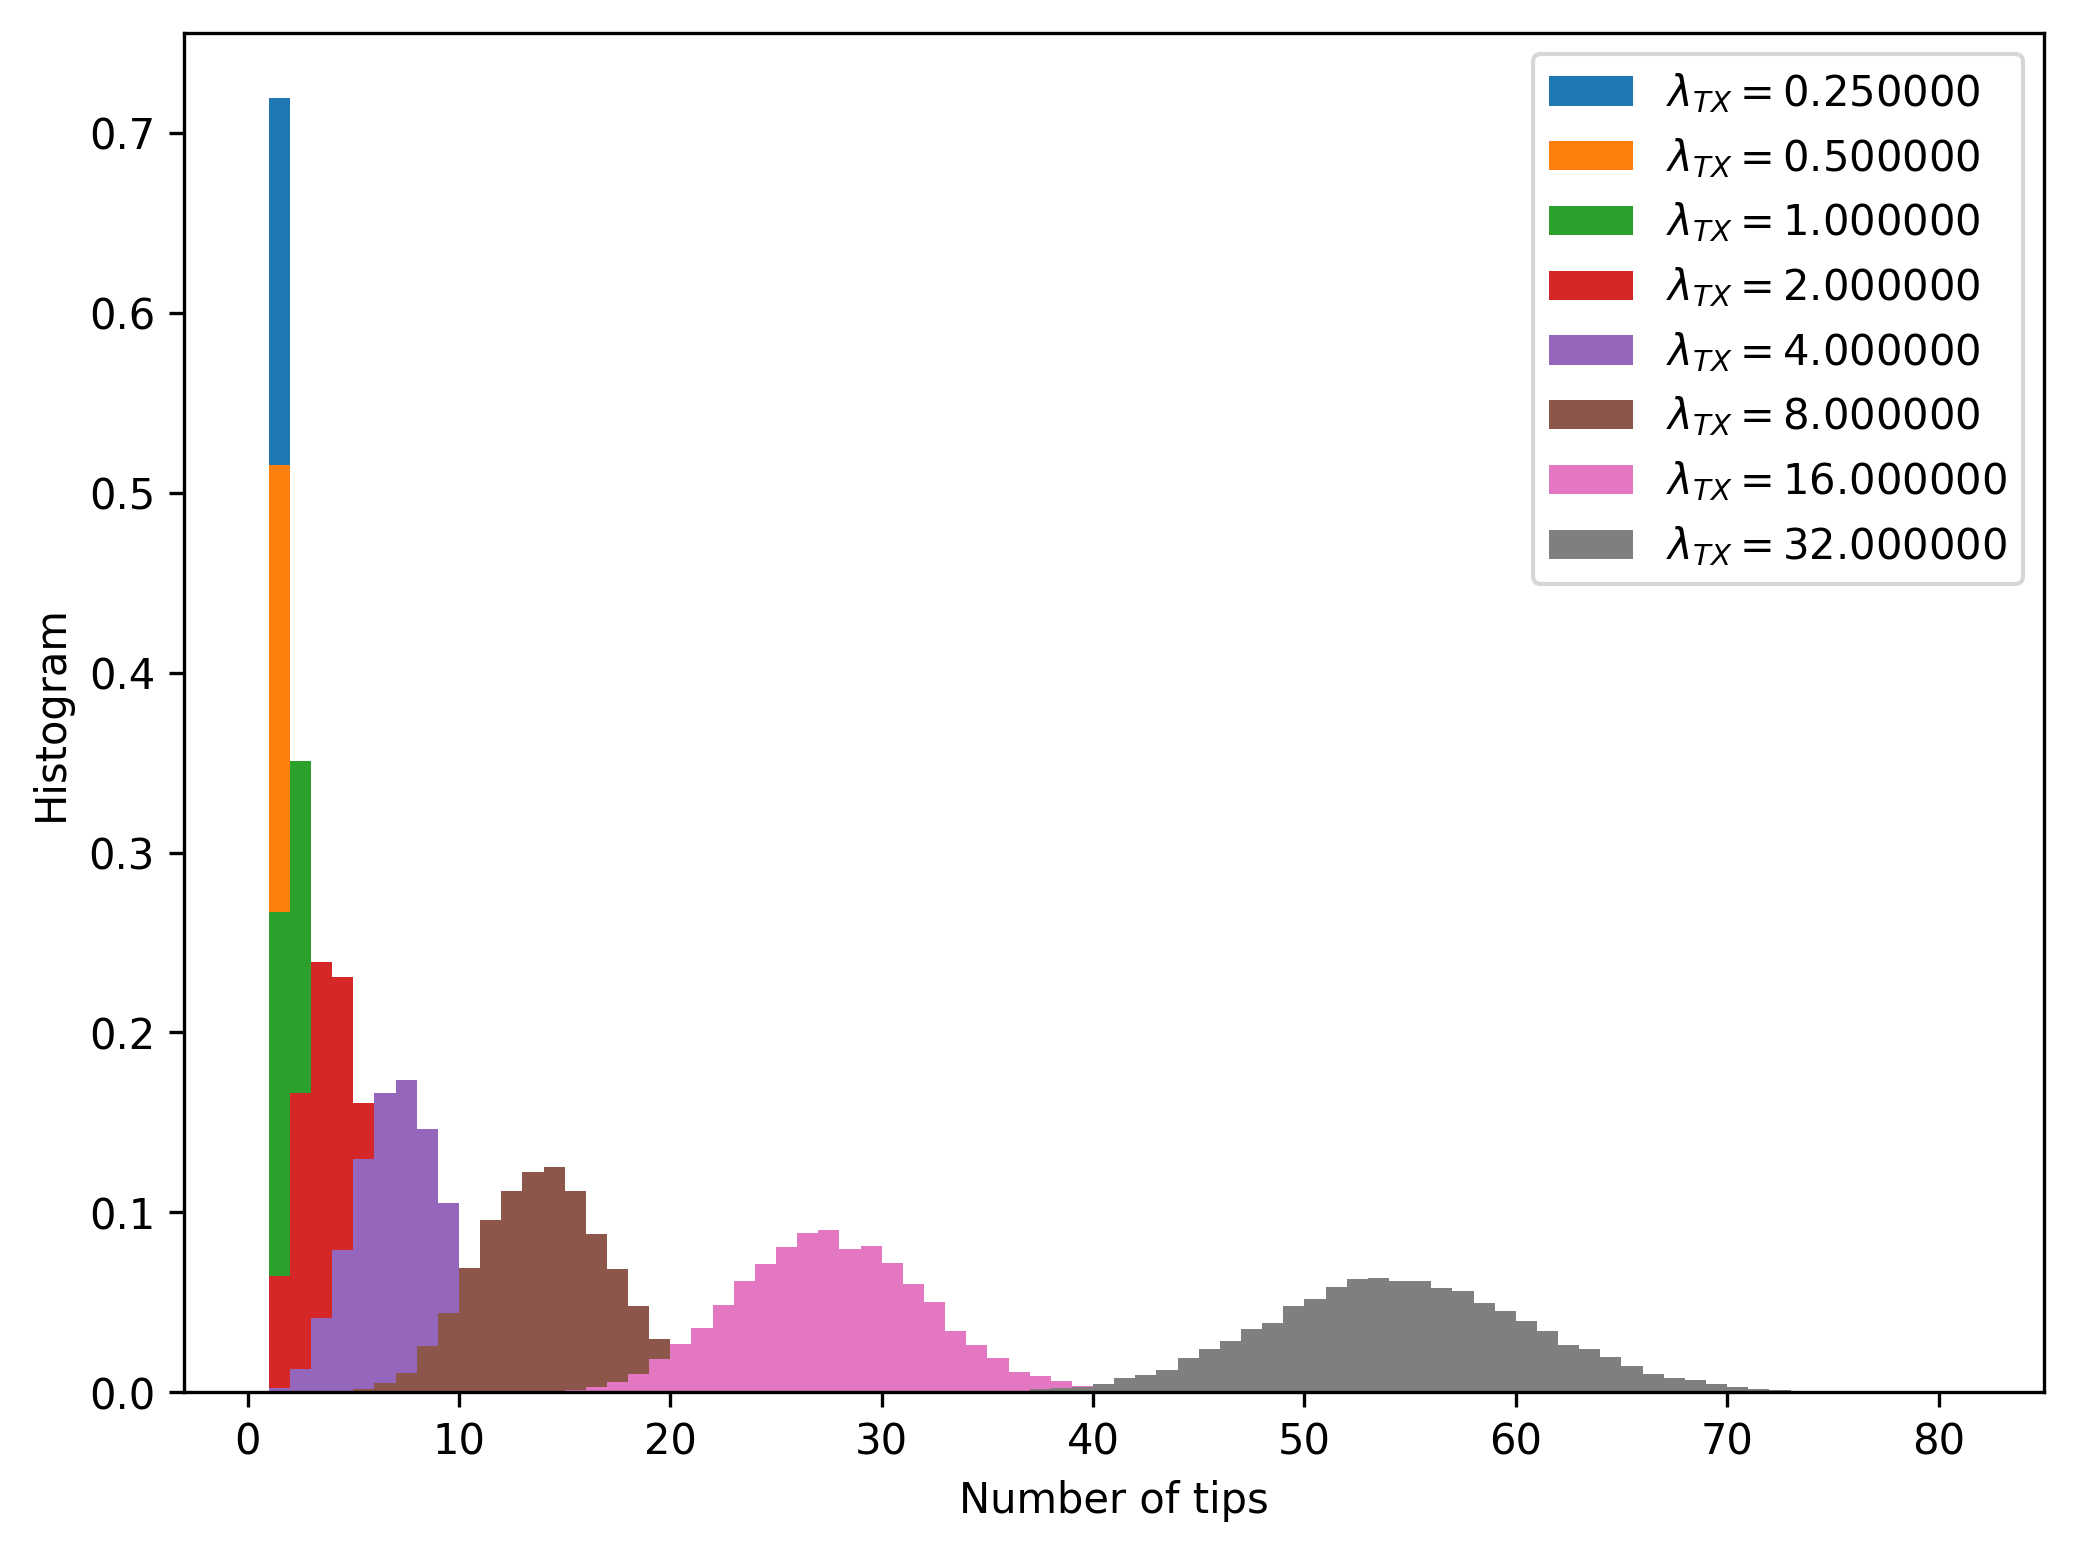
\includegraphics[width=0.7\textwidth]{./images01/new2/tips_aggregate.png}
\caption{Histogram of the number of tips for different load scenarios.}
\end{figure}
\end{frame}


%=============================================
%=============================================
%=============================================


\section{An invitation to Sparse Distributed Memory: from the theoretical model to the system dynamics}
\begin{frame}
\sectionpage
\end{frame}


\begin{frame}
\frametitle{An invitation to Sparse Distributed Memory: from the theoretical model to the system dynamics}

SDM is a mathematical \textbf{model of long-term memory} that has a number of neuroscientific and psychologically plausible dynamics.

This model is used in all sort of applications due to its ability to closely reflect \textbf{the human capacity to remember past experiences}.

This flexibility into \textbf{mapping one situation in another} is an essential human feature which is hard to replicate in computers.

\end{frame}


\begin{frame}
\frametitle{SDM: How does it work?}

\begin{figure}
\centering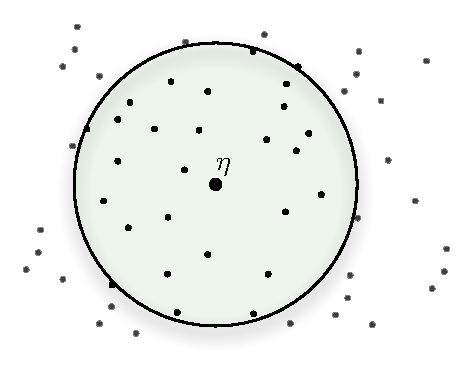
\includegraphics[scale=0.75]{./images02/p_circle_r.pdf}
\caption{Activated addresses inside access radius $r$ around the center address.}
\end{figure}

\end{frame}


\begin{frame}
\frametitle{SDM: How does it work?}
\begin{figure}
\centering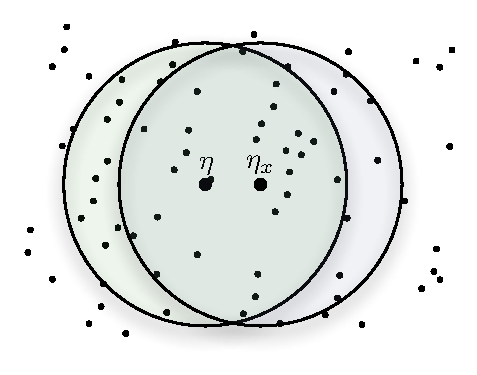
\includegraphics[scale=0.75]{./images02/p1_inter_p2.pdf}
\caption{Shared addresses between the target datum $\eta$ and the cue $\eta_{x}$.}
\end{figure}
\end{frame}


\begin{frame}
\frametitle{SDM: How does it work?}
\begin{figure}
\centering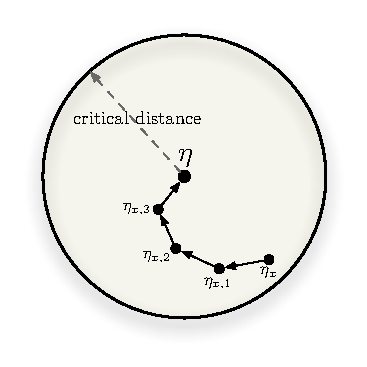
\includegraphics[scale=0.75]{./images02/p1_p2_iter_read.pdf}
\caption{In this example, four iterative readings were required to converge from $\eta_{x}$ to $\eta$.}
\end{figure}
\end{frame}


\begin{frame}
\frametitle{SDM: How does it work?}
\begin{figure}
\centering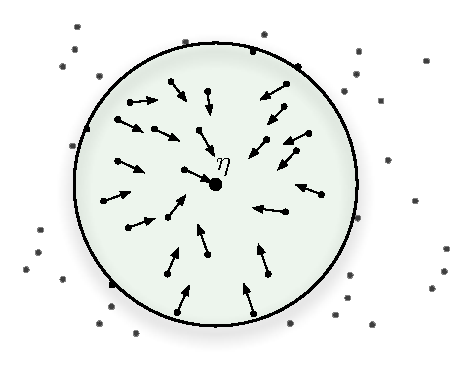
\includegraphics[scale=0.75]{./images02/p1_after_write.pdf}
\caption{Hard-locations pointing, approximately, to the target bitstring.}
\end{figure}
\end{frame}

\begin{frame}
\frametitle{Contributions}

The main contributions are:
\begin{enumerate}[i]
\item A validated, open-source, cross-platform framework in which researchers are able to replicate someone else's results
\item Identification and modeling of the autocorrelation in the counters
\item Loss of neurons resilience
\item Noise filtering application
\item Classification application
\item Reinforcement learning application
\end{enumerate}
\end{frame}


\begin{frame}
\frametitle{Loss of neurons resilience}
\begin{figure}
\centering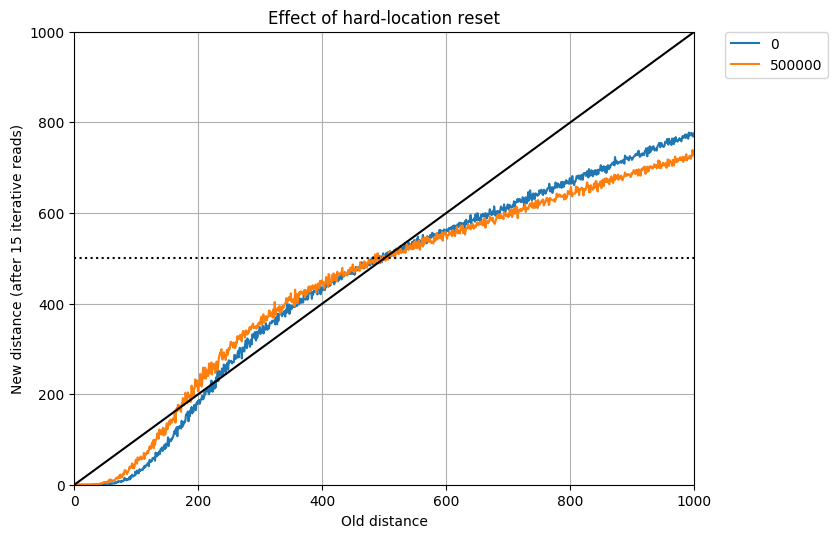
\includegraphics[width=0.7\textwidth]{./images02/new-images/sdm-neuron-death-500k.png}
\caption{This graph shows the SDM's robustness against loss of neurons in a SDM with $n=1,000$ and $H=1,000,000$. Even when 50\% of neurons are dead, SDM recall is barely affected, which is an impressive result and matches with some clinical results of children submitted to hemispherectomy.
\label{fig:sdm-neuron-death-500k}}
\end{figure}
\end{frame}


\begin{frame}
\frametitle{Loss of neurons resilience}
\begin{figure}
\centering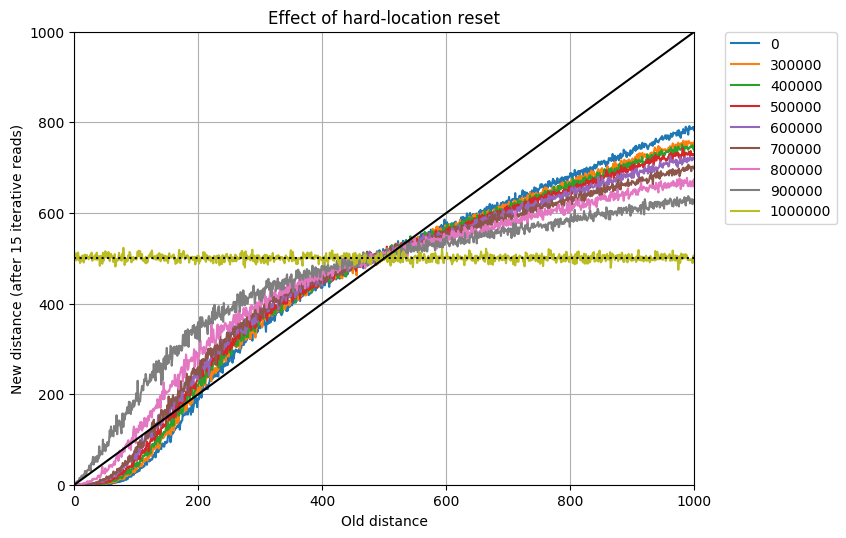
\includegraphics[width=0.7\textwidth]{./images02/new-images/sdm-neuron-death-1m.png}
\caption{This graph shows the SDM's robustness against loss of neurons in a SDM with $n=1,000$ and $H=1,000,000$. The more neurons are lost, the smaller the critical distance, i.e., the worse the SDM recall.
\label{fig:sdm-neuron-death-1m}}
\end{figure}
\end{frame}


\begin{frame}
\frametitle{Critical distance \& Autocorrelation}
\begin{figure}
\subfloat{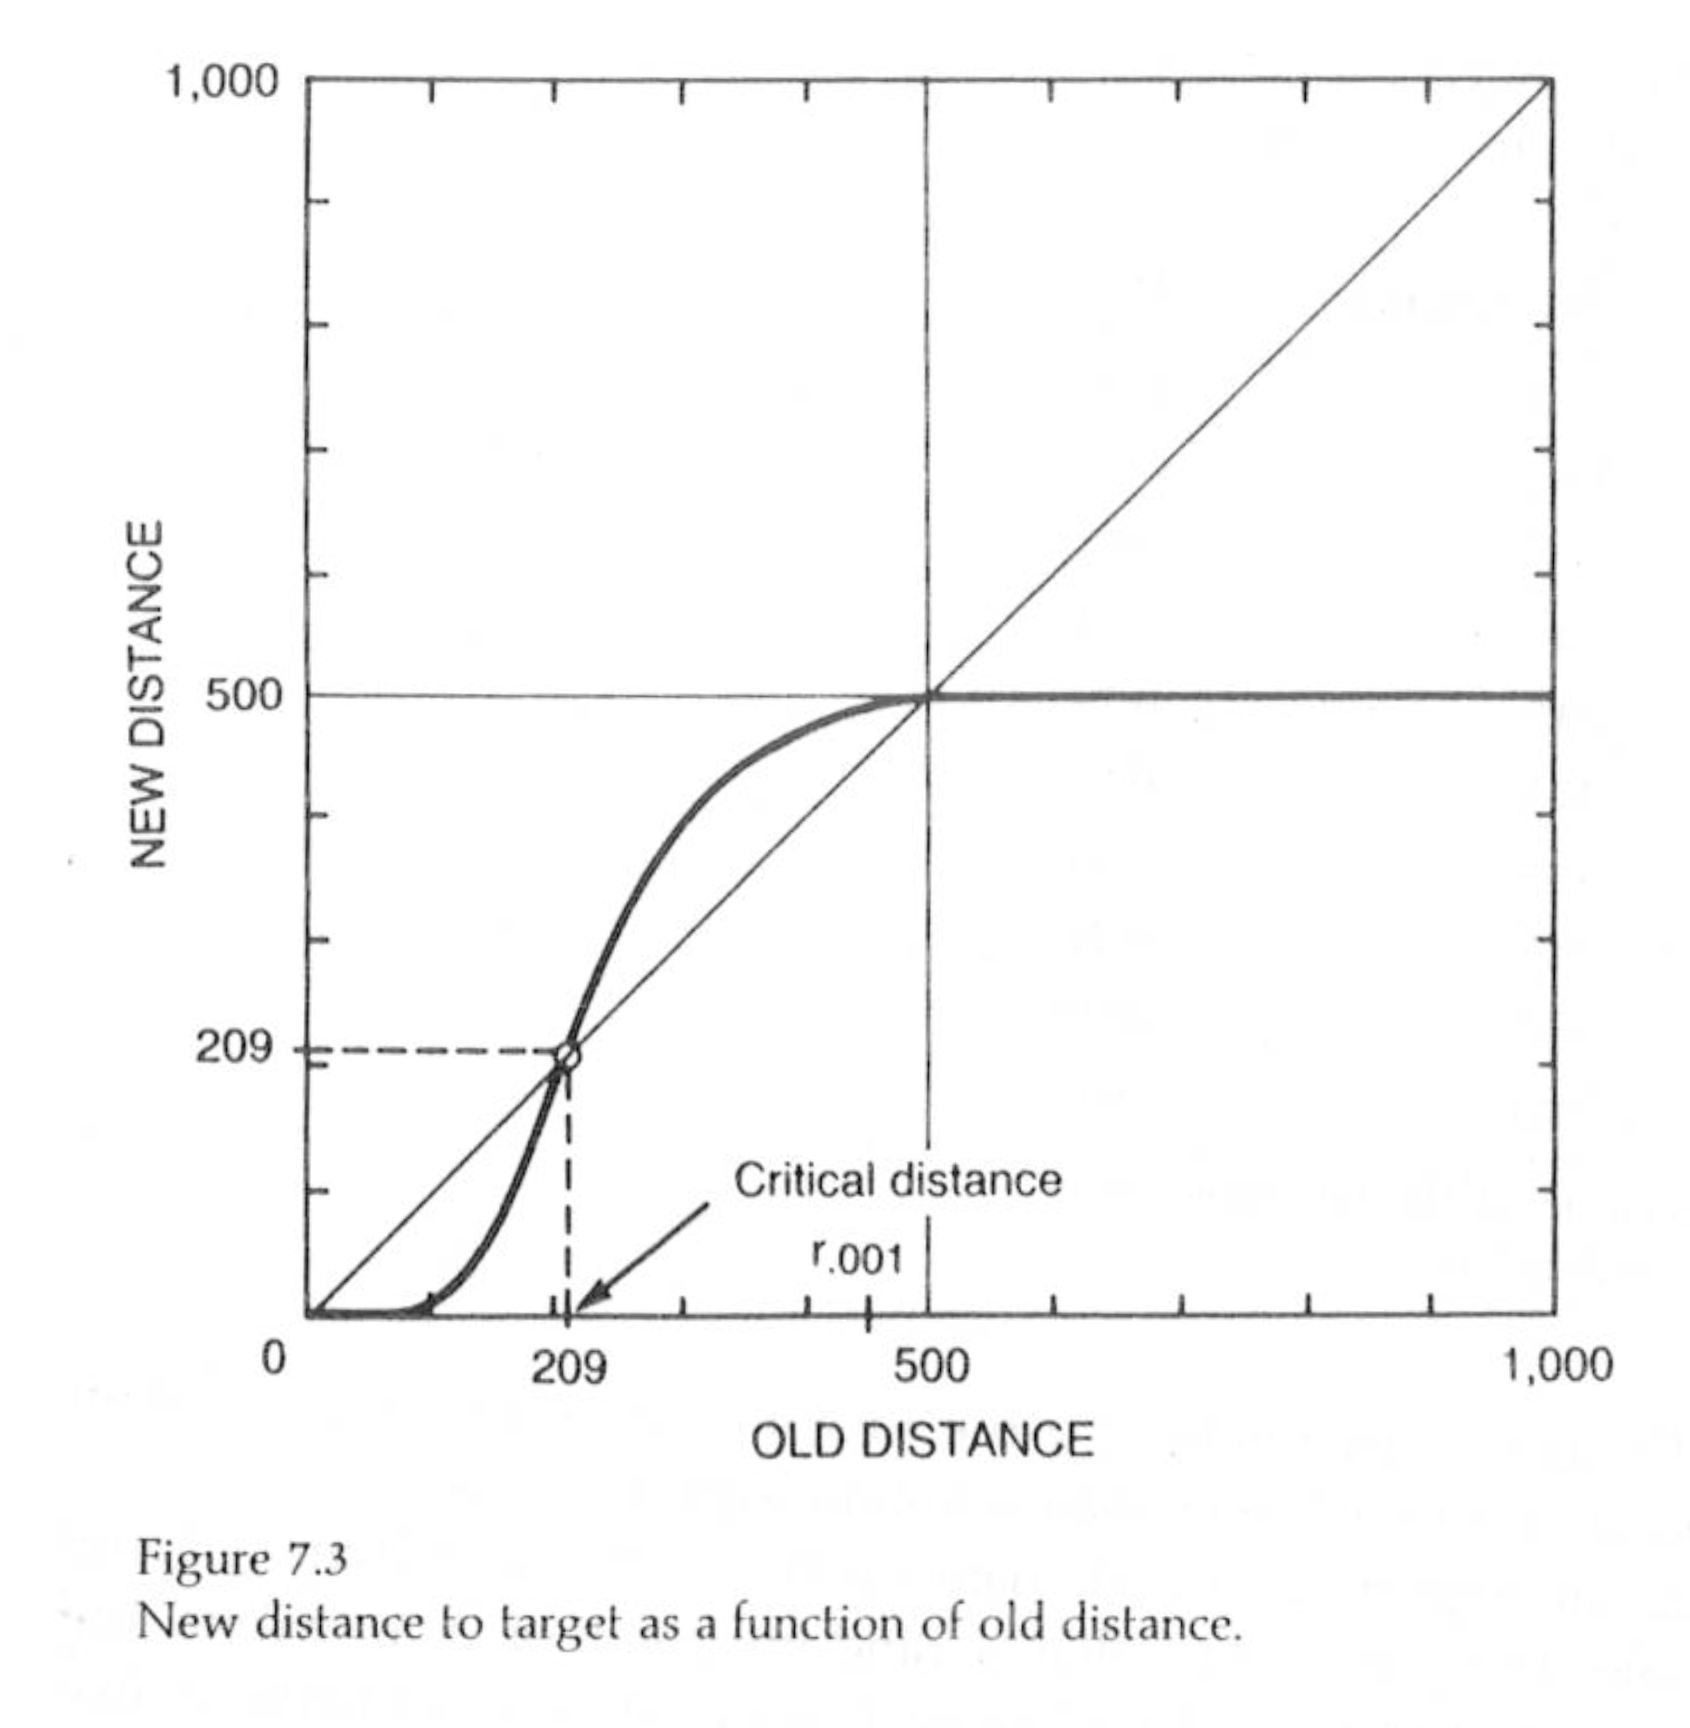
\includegraphics[width=0.46\textwidth,valign=t]{./images02/kanerva-table-7-2-original.png}}
\subfloat{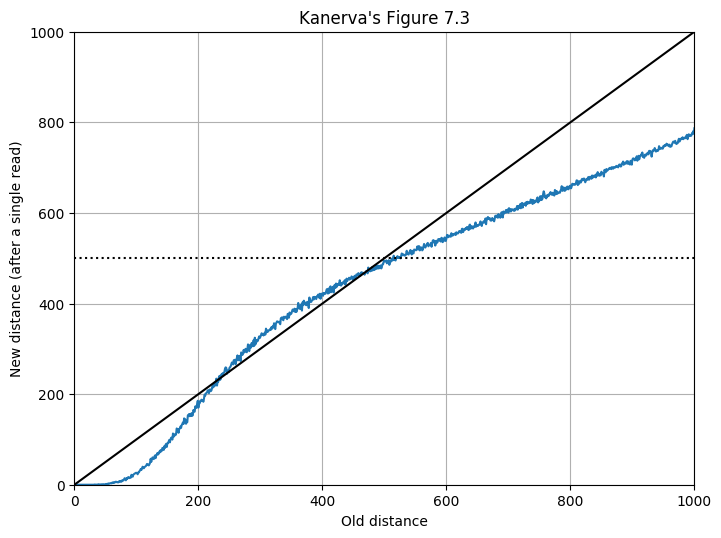
\includegraphics[width=0.54\textwidth,valign=t]{./images02/sdm-10000w-table-7-2-6-samples.png}}
\end{figure}
\end{frame}


\begin{frame}
\frametitle{Critical distance \& Autocorrelation}
\begin{theorem}
\emph{Each dimension has a small pull bias, which can be measured by}
$P(x_i = y_i | d(x, y) \le r) = \dfrac{\sum_{k=0}^{r} \binom{n-1}{k}}{\sum_{k=0}^{r} \binom{n}{k}}$
\end{theorem}

\begin{theorem}
The autocorrelation vanishes when $n \rightarrow \infty$, i.e., $\lim_{n \rightarrow \infty} P(x_i = y_i | d(x, y) \le r) = 1/2$.
\end{theorem}

When $n=1,000$ and $r=451$, $P(x_i = y_i | d(x, y) \le r) = 0.552905498137$.
\end{frame}


\begin{frame}
\frametitle{Critical distance \& Autocorrelation}
\begin{figure}
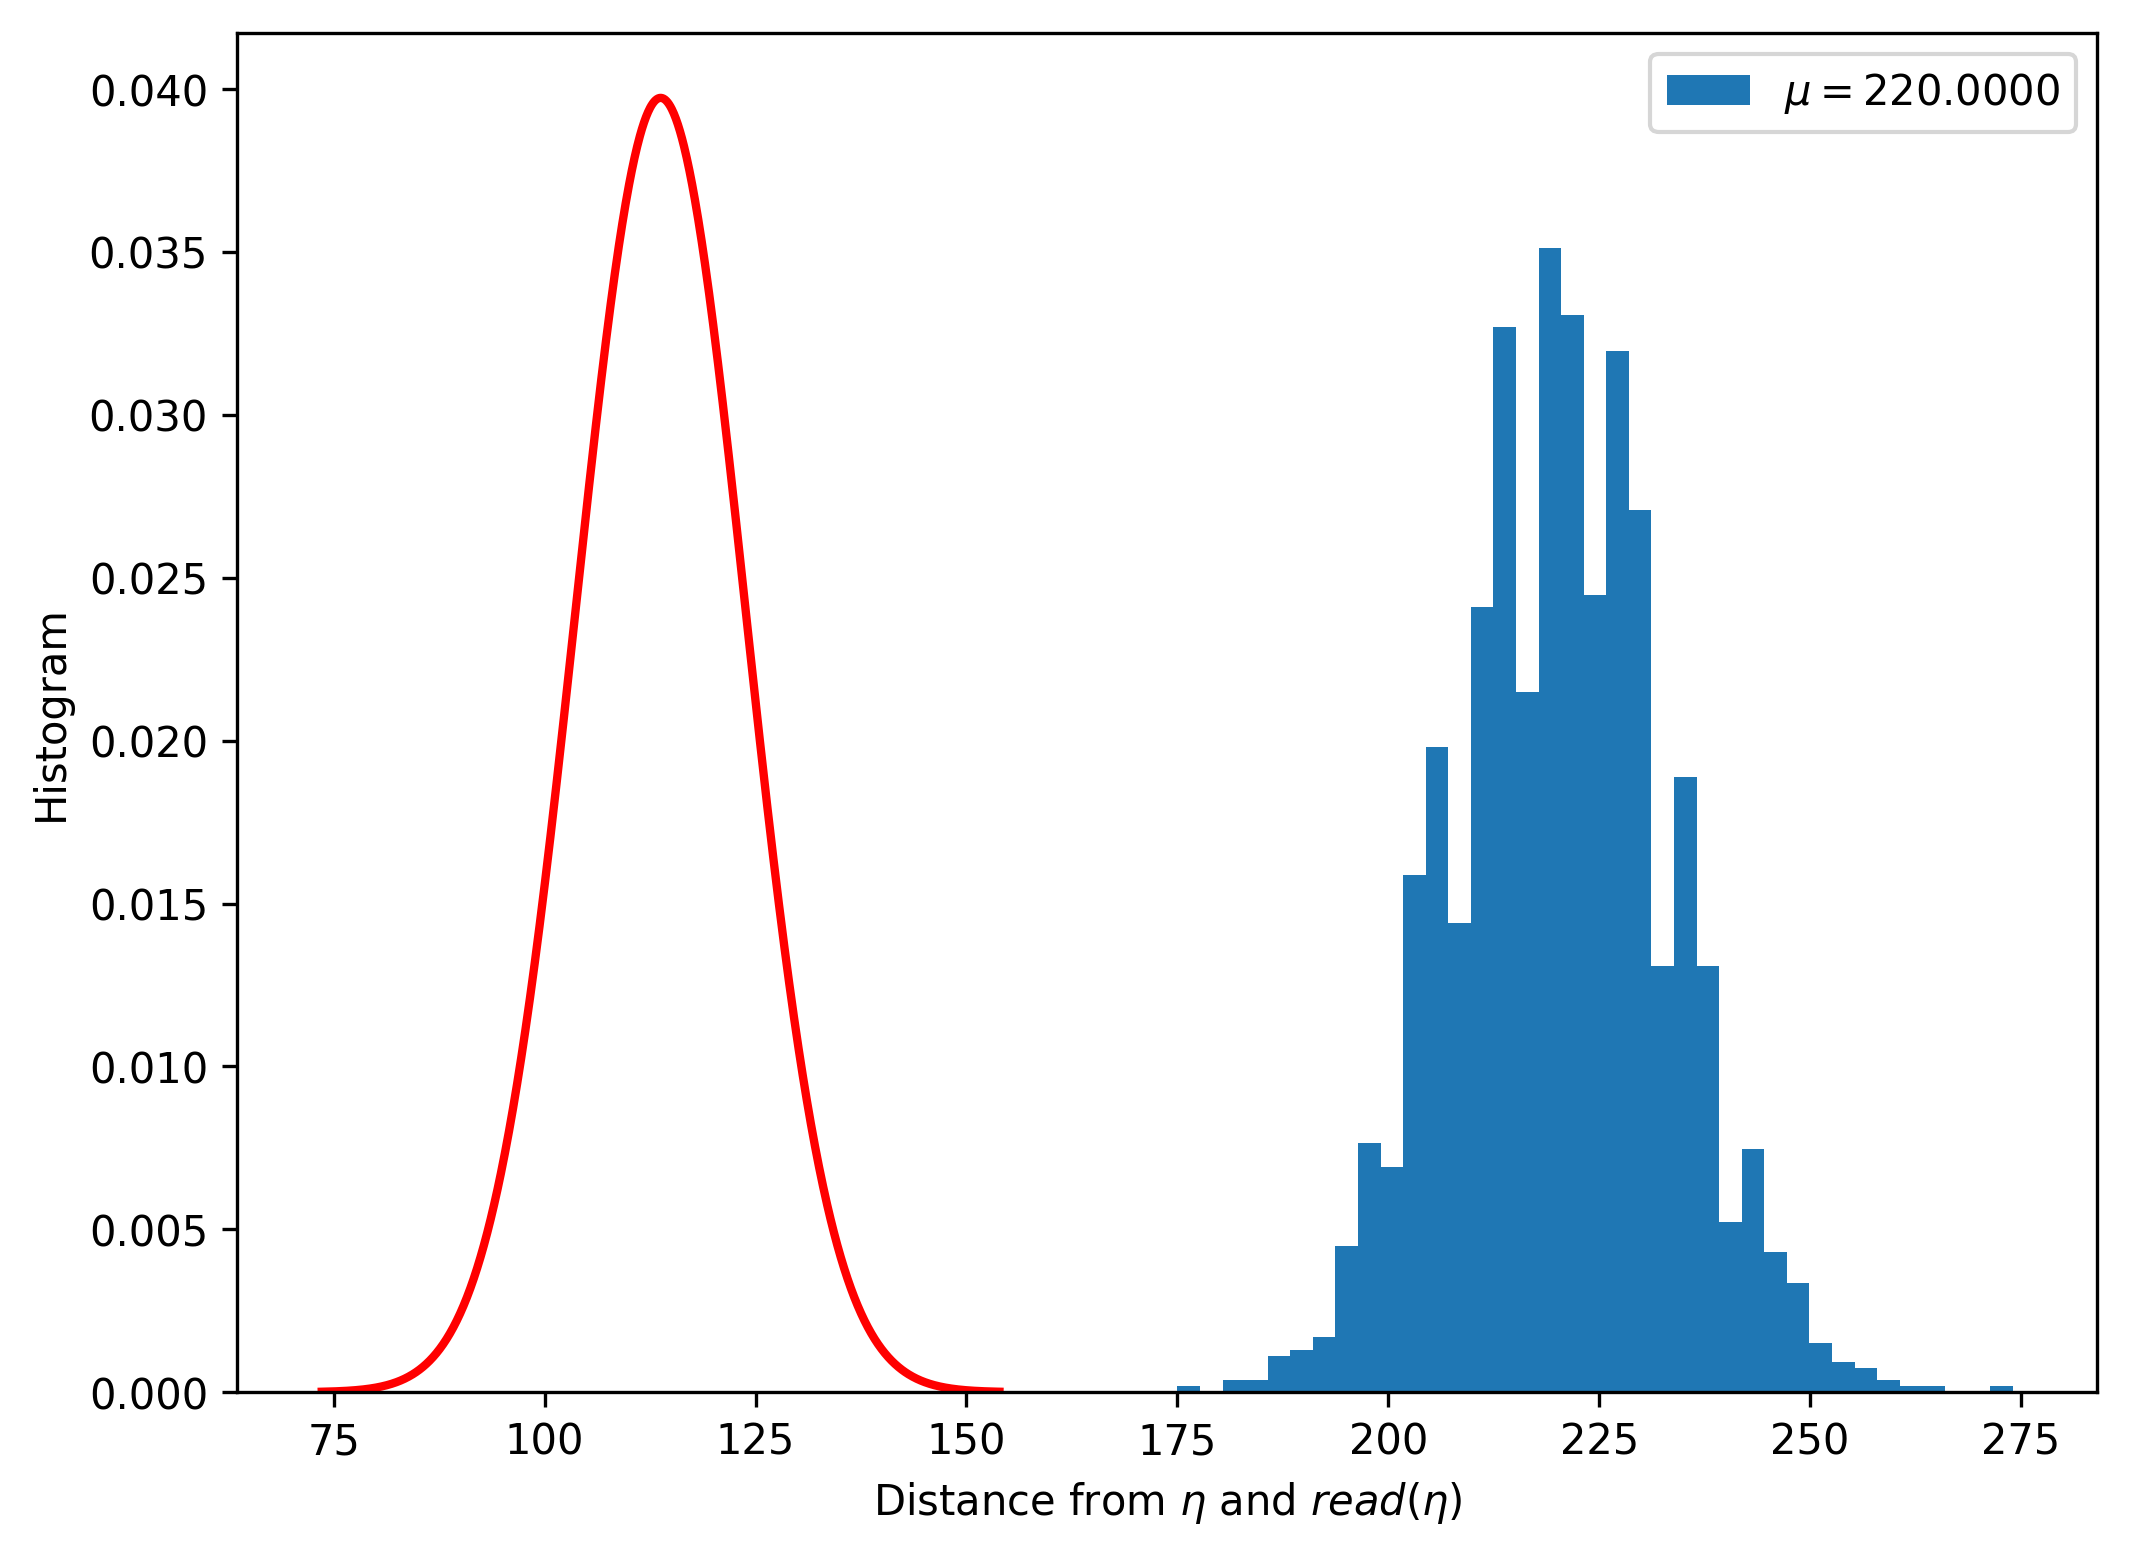
\includegraphics[width=0.75\textwidth]{./images02/autocorrelation/read-random-bs.png}
\caption{The histogram was obtained through simulation. The red curve is the theoretical normal distribution.}
\end{figure}
\end{frame}


\begin{frame}
\frametitle{Critical distance \& Autocorrelation}
The analytical model which does not consider autocorrelation predicts a critical distance of 209 bits.

\begin{figure}
\centering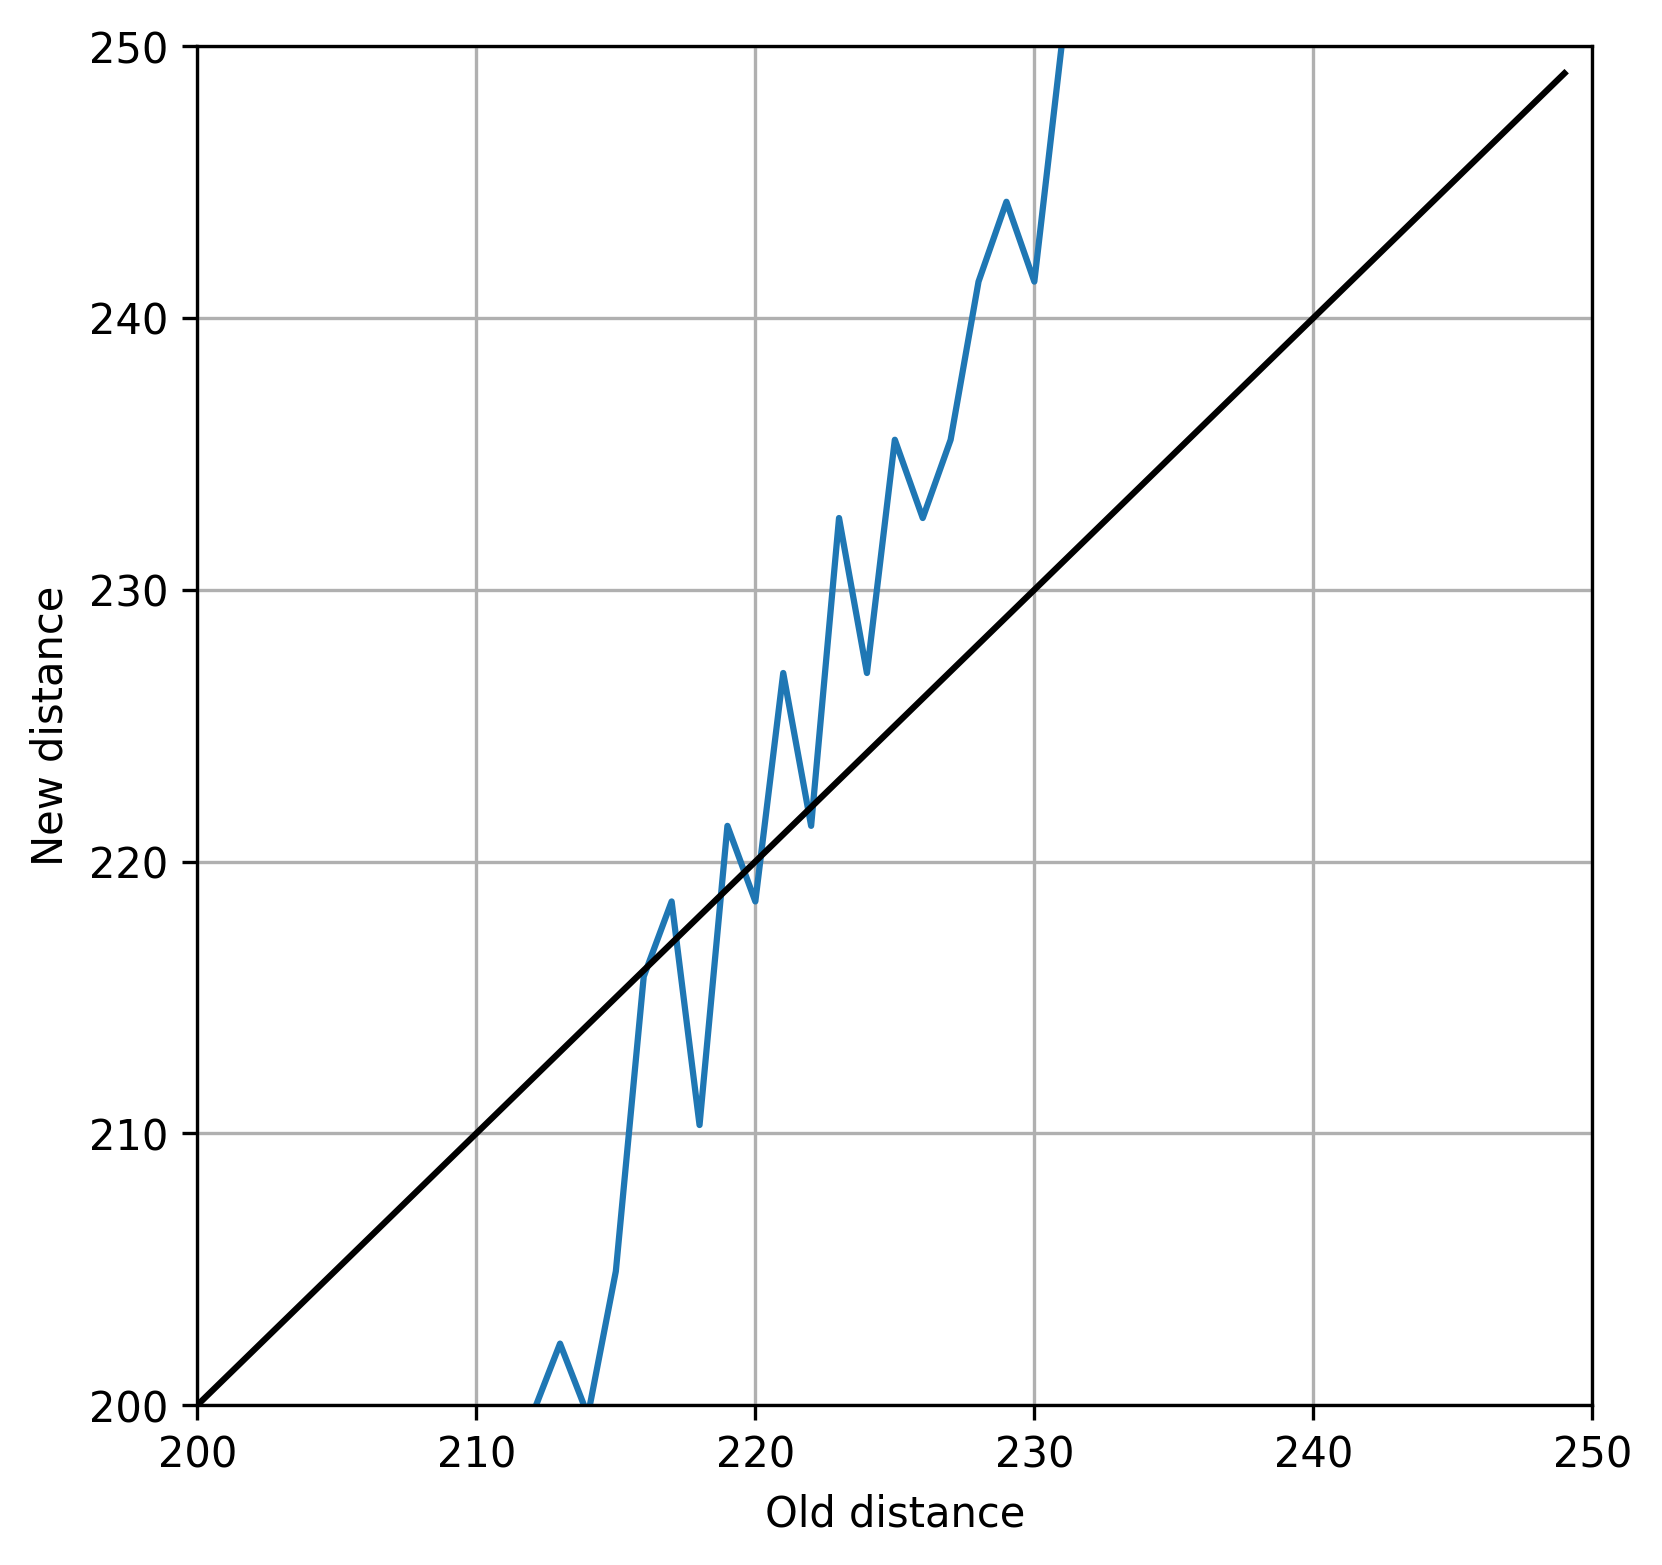
\includegraphics[width=0.5\textwidth]{./images02/figure-73-eq-zoom.png}
\caption{Zoom-in around $d=209$.}
\end{figure}
\end{frame}


\begin{frame}
\frametitle{Classification application: Training}
\begin{figure}
\centering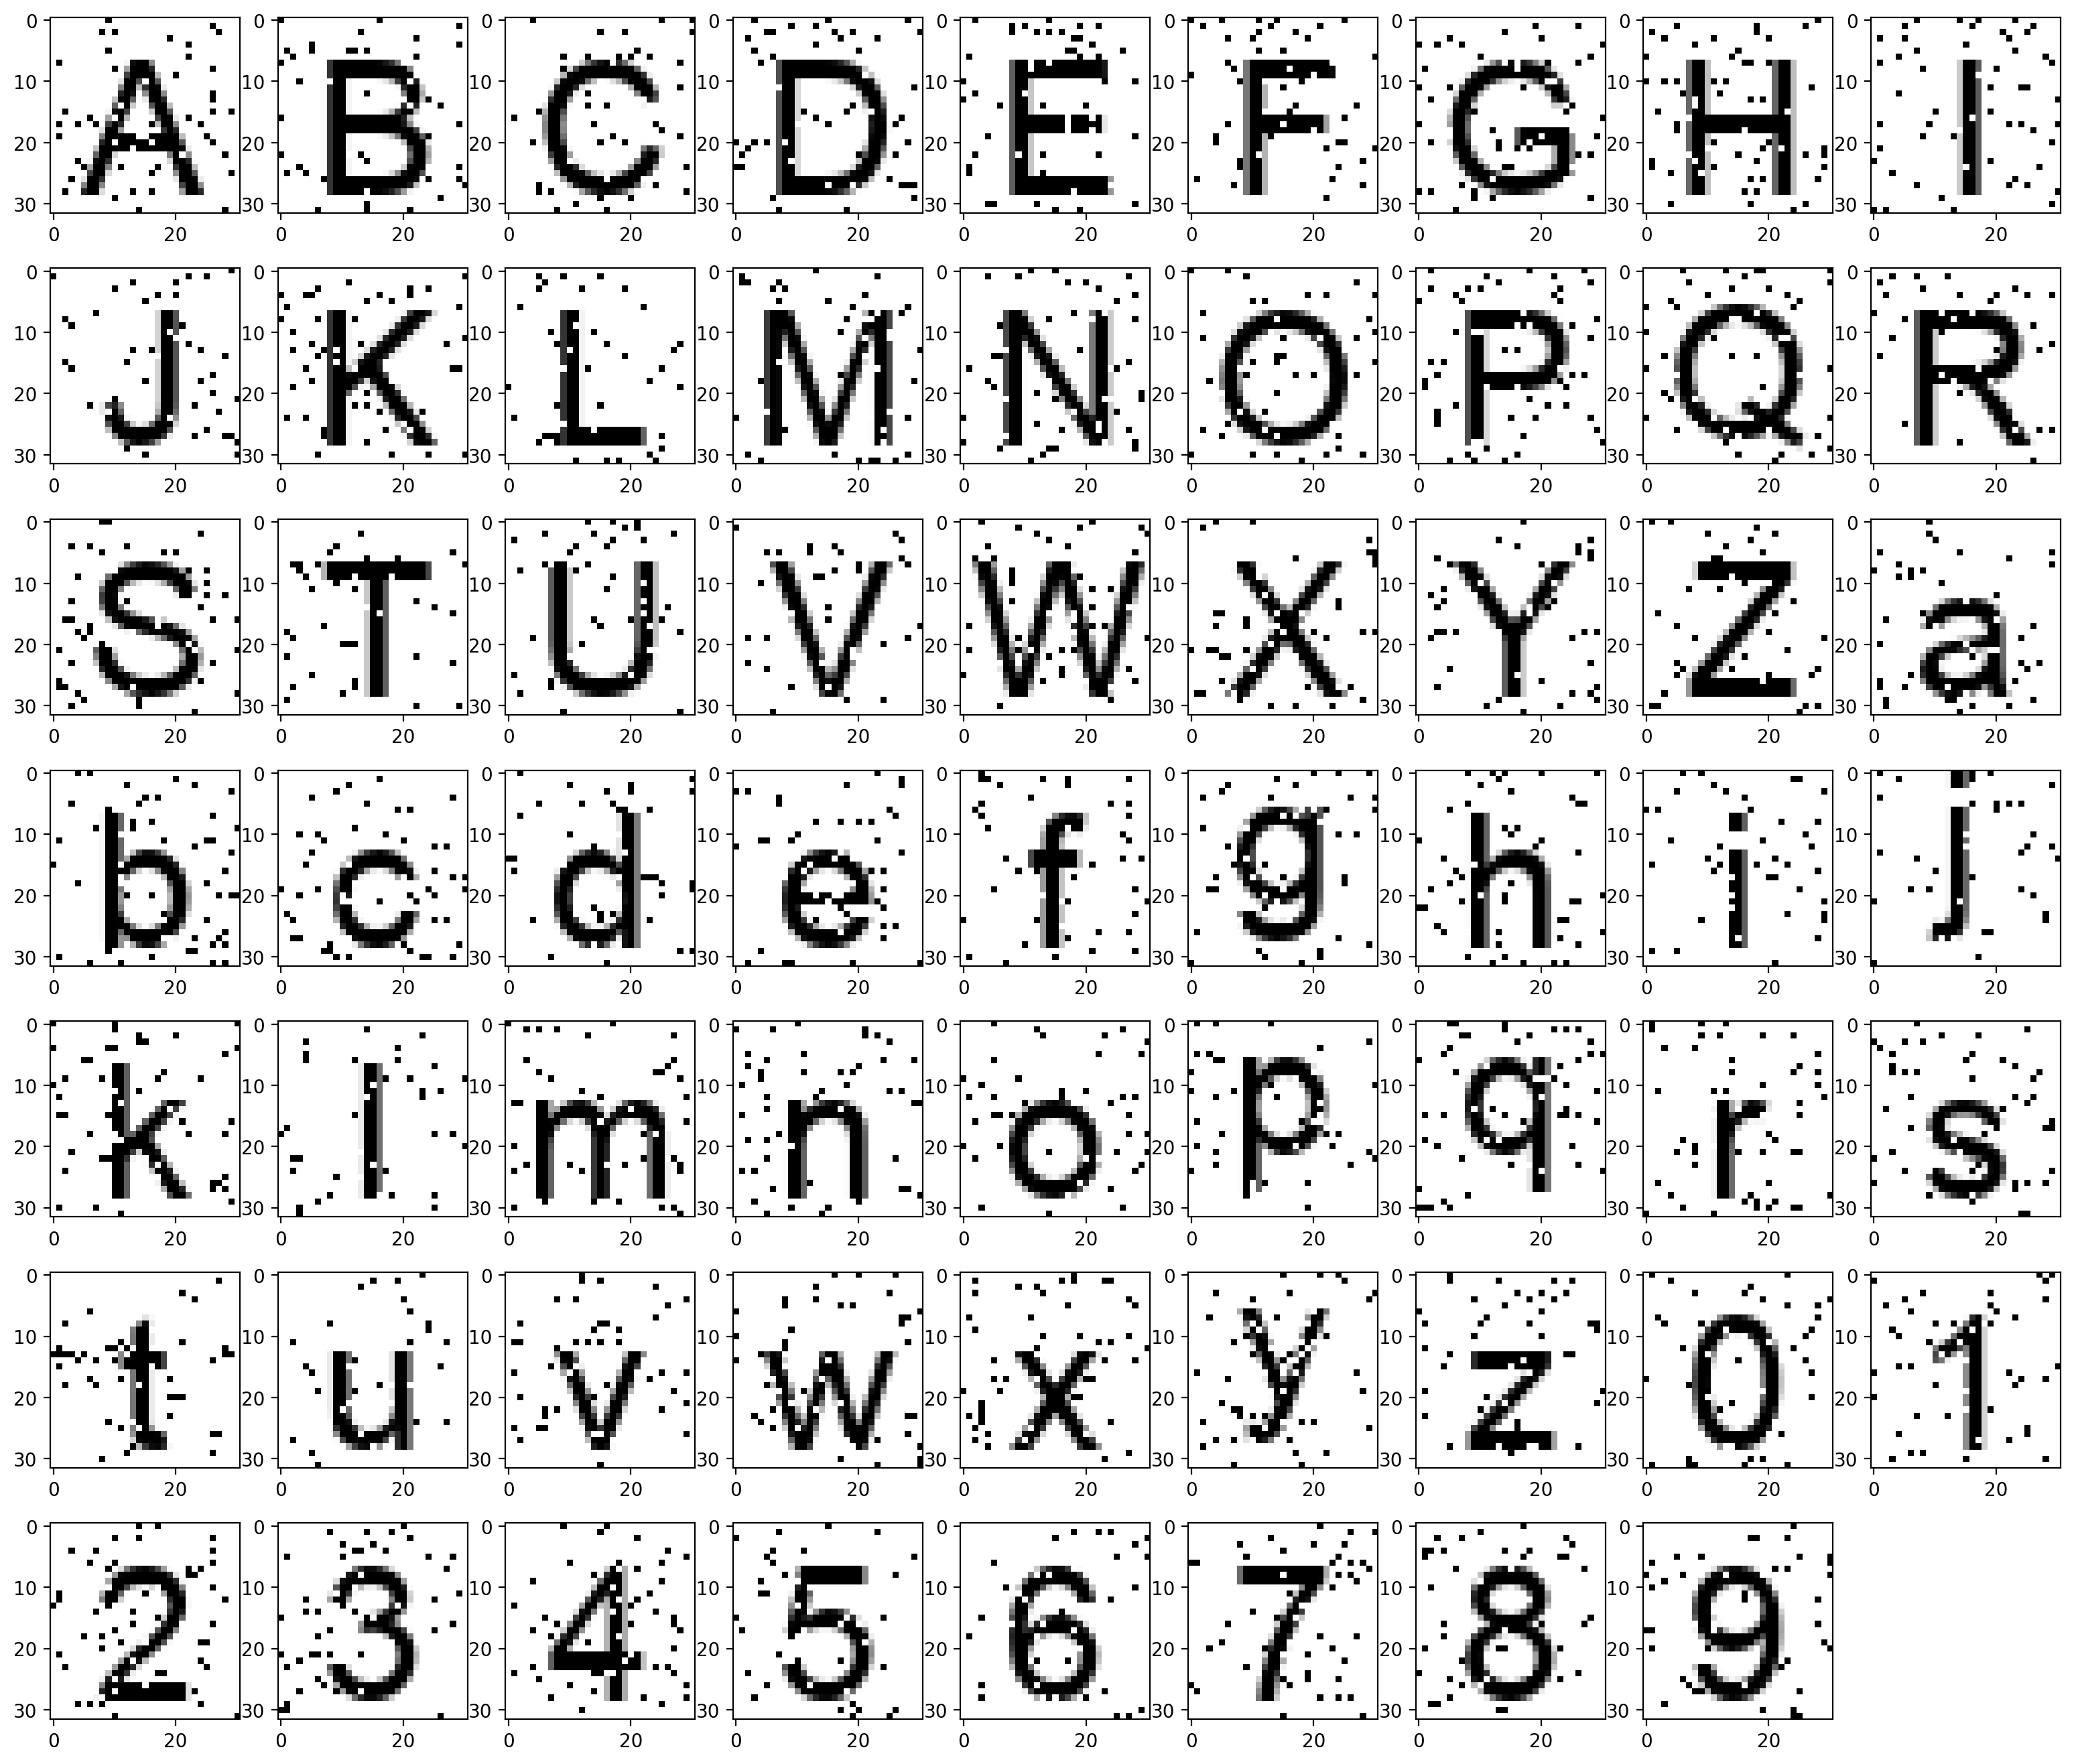
\includegraphics[width=0.6\textwidth]{./images02/classification/groups.png}
\caption{One noisy image for each of the 62 classification groups.
\label{fig-classification-groups}}
\end{figure}
\end{frame}

\begin{frame}
\frametitle{Classification application: Confusing cases}
\begin{figure}
  \centering
  \subfloat[``i'', ``l'', and ``r'' with 20\% noise.]{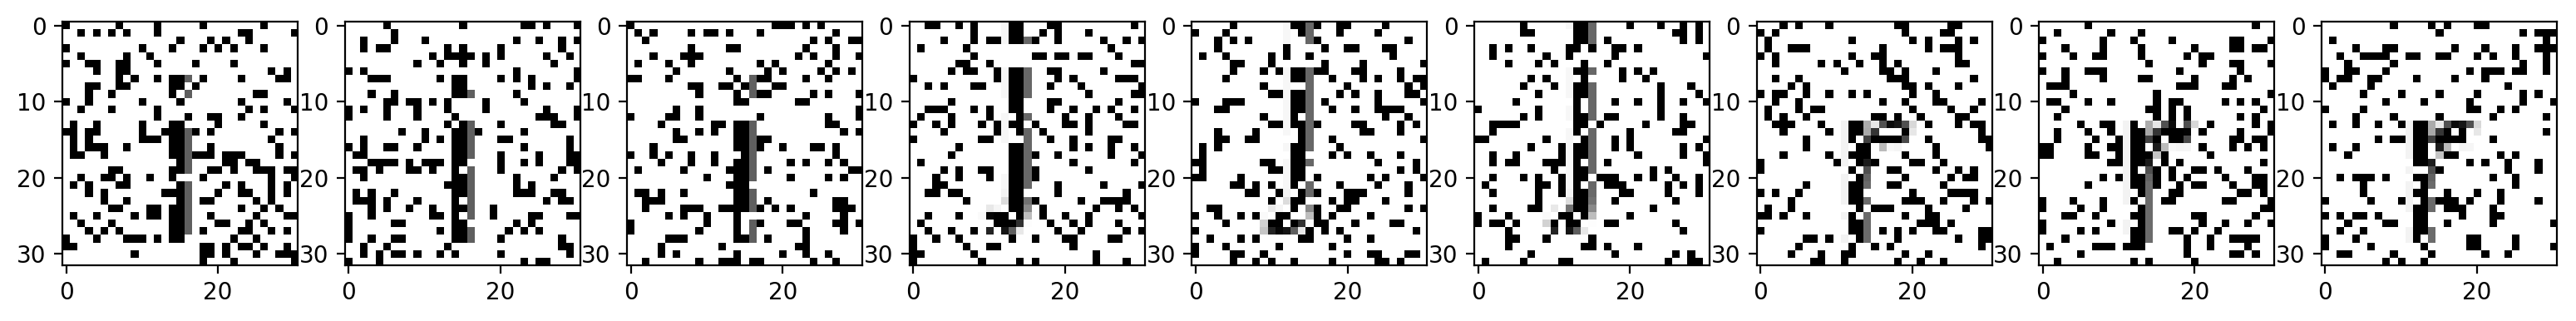
\includegraphics[width=\textwidth]{./images02/classification/ilr-high-noise.png}}

  \subfloat[``i'', ``l'', and ``r'' with 5\% noise.]{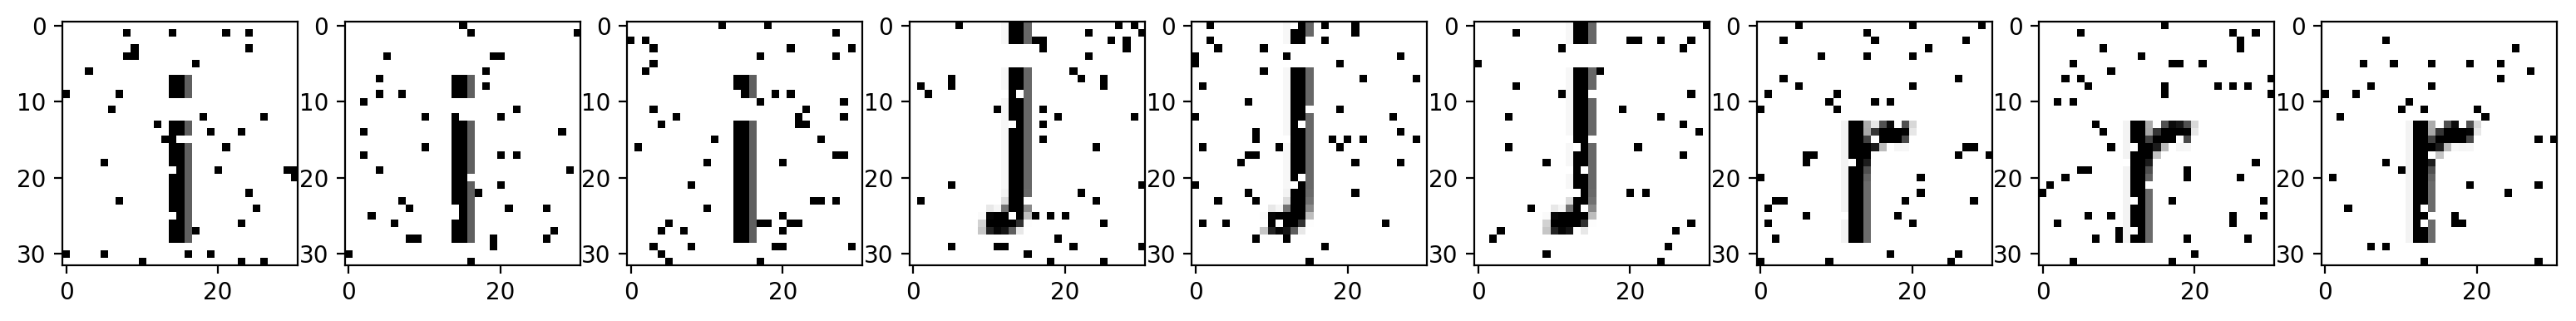
\includegraphics[width=\textwidth]{./images02/classification/ilr-low-noise.png}}

\end{figure}
\end{frame}


\begin{frame}
\frametitle{Classification application: Confusing cases (2)}
\begin{figure}
  \centering
  \subfloat[``c'', ``d'', and ``o'' with 20\% noise.]{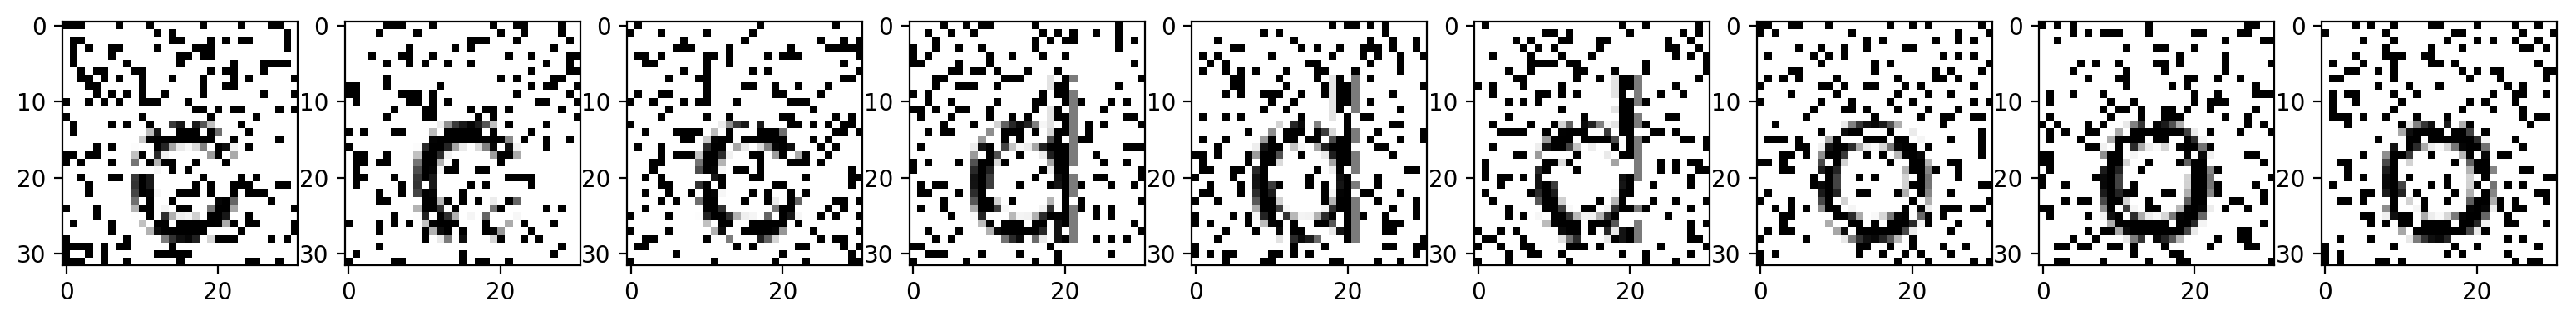
\includegraphics[width=\textwidth]{./images02/classification/cdo-high-noise.png}}

  \subfloat[``c'', ``d'', and ``o'' with 5\% noise.]{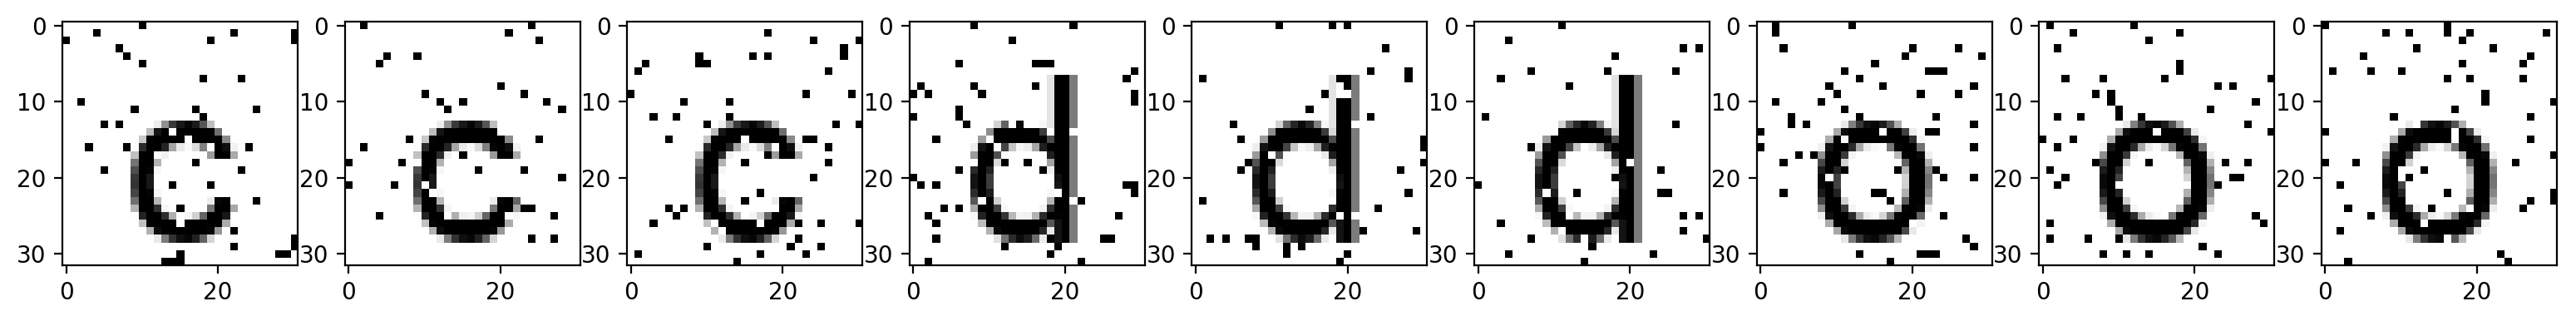
\includegraphics[width=\textwidth]{./images02/classification/cdo-low-noise.png}}

\end{figure}
\end{frame}


\begin{frame}
\frametitle{Classification application: Confusing cases (3)}
\begin{figure}
  \centering
  \subfloat[``G'', ``O'', and ``Q'' with 20\% noise.]{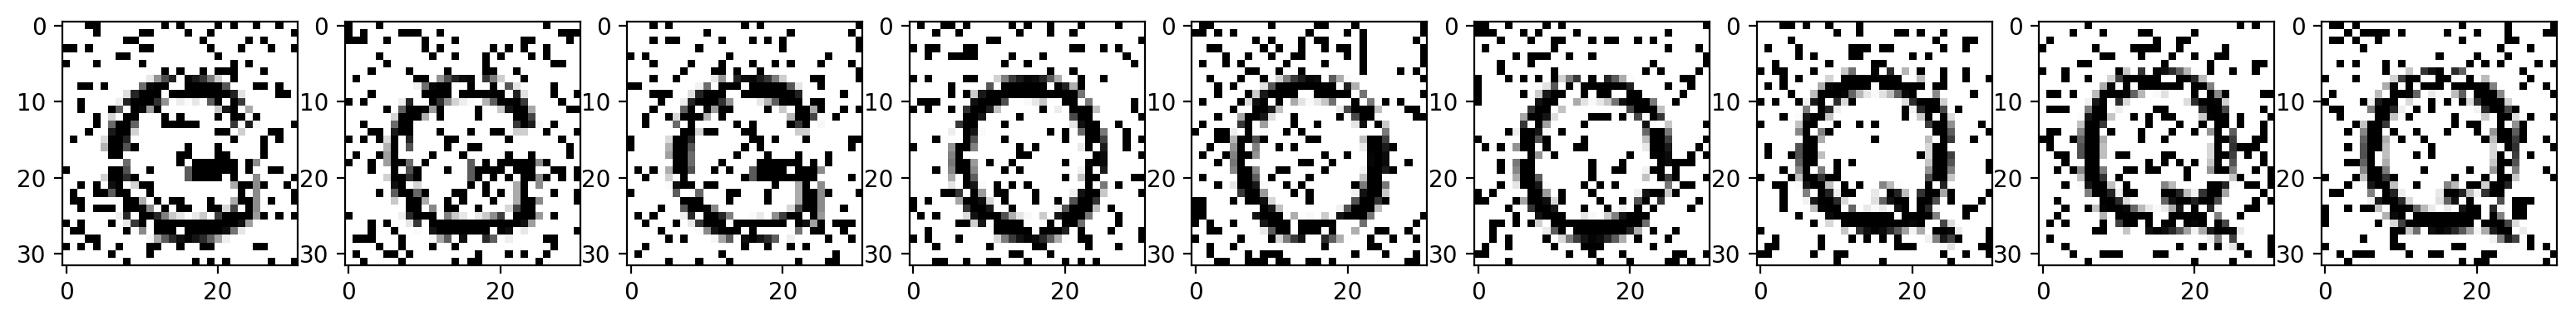
\includegraphics[width=\textwidth]{./images02/classification/GOQ-high-noise.png}}

  \subfloat[``G'', ``O'', and ``Q'' with 5\% noise.]{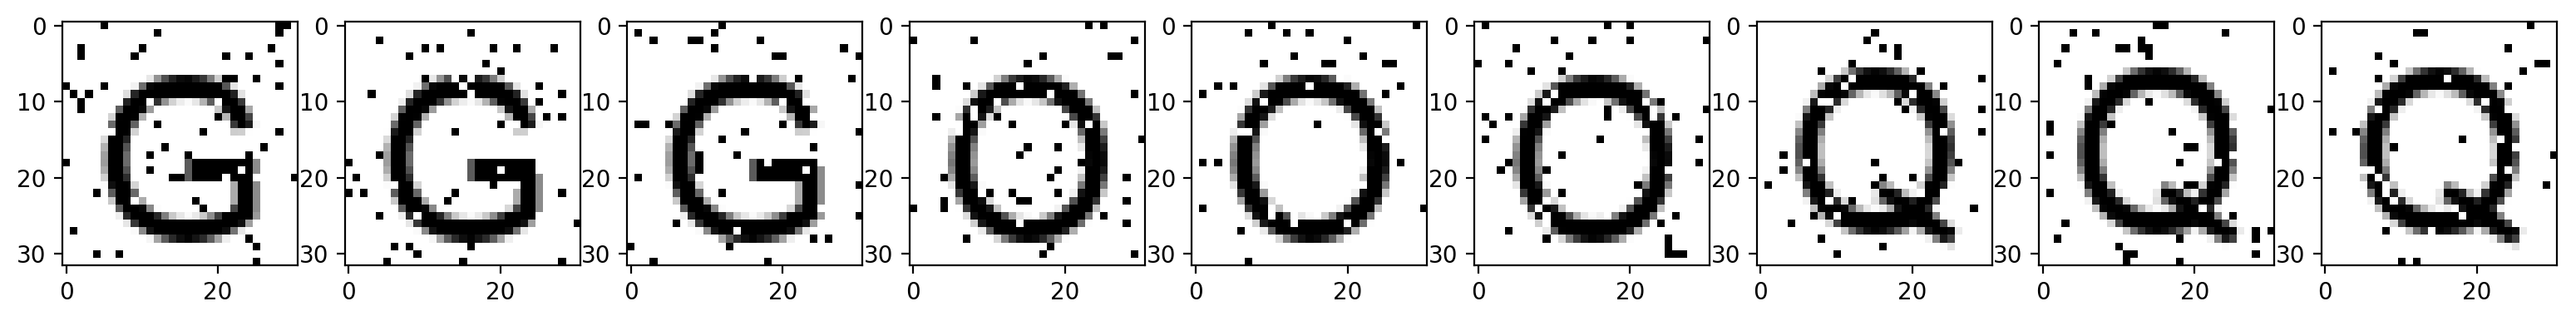
\includegraphics[width=\textwidth]{./images02/classification/GOQ-low-noise.png}}

\end{figure}
\end{frame}


\begin{frame}
\frametitle{Classification application: Results}
Generally speaking, the classification algorithm made some mistakes in the 20\% noise scenario, and just a few mistakes in the 5\% noise scenario.

When the training set has 1,000 samples (instead of 100) of each letter, the algorithm correctly classify almost all letters in both 20\% and 5\% noise scenarios, except for letters ``e'' and ``o''.

It seems that the algorithm could not differentiate letters ``e'' and ``o'' because their differences are \textbf{smaller than the critical distance}. I believe it would just have to be trained more and more in order to learn to differentiate them (because the critical distance decreases when more items are written into the memory).
\end{frame}


\begin{frame}
\frametitle{Noise filtering: Interference}
\begin{figure}
\includegraphics[height=0.15\textheight]{./images02/filter/case2-b-10noise.png}
\end{figure}
\begin{figure}
\includegraphics[height=0.15\textheight]{./images02/filter/case2-c-10noise.png}
\end{figure}
\begin{figure}
\includegraphics[height=0.15\textheight]{./images02/filter/case2-d-10noise.png}
\end{figure}
\begin{figure}
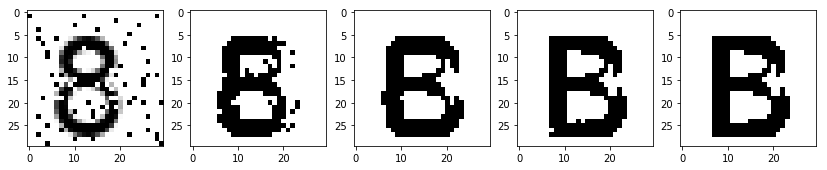
\includegraphics[height=0.15\textheight]{./images02/filter/case2-8-10noise.png}
\end{figure}
\end{frame}


\begin{frame}
\frametitle{Noise filtering: After using labels}
\begin{figure}
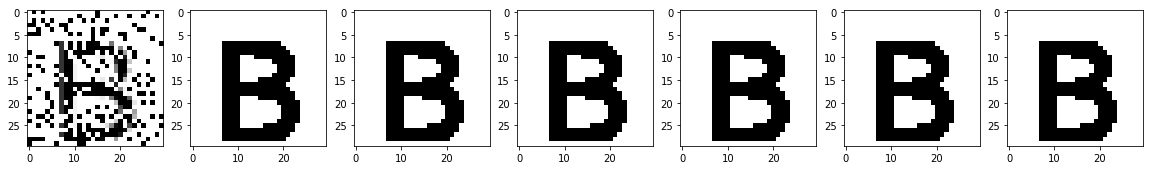
\includegraphics[width=0.5\textwidth]{./images02/filter/labelB-20noise.png}
\end{figure}
\begin{figure}
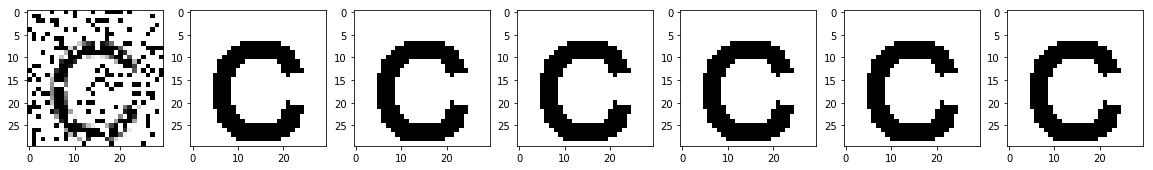
\includegraphics[width=0.5\textwidth]{./images02/filter/labelC-20noise.png}
\end{figure}
\begin{figure}
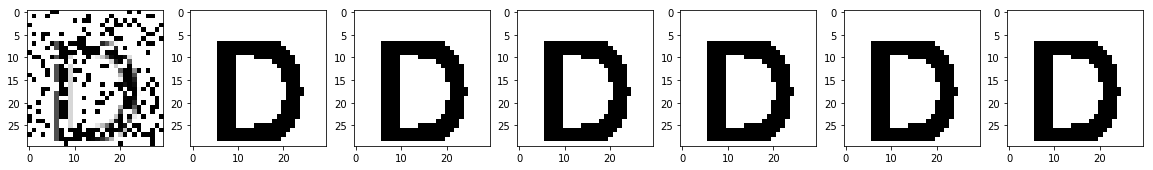
\includegraphics[width=0.5\textwidth]{./images02/filter/labelD-20noise.png}
\end{figure}
\begin{figure}
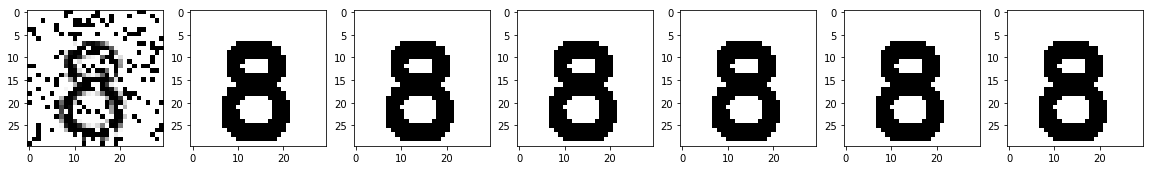
\includegraphics[width=0.5\textwidth]{./images02/filter/label8-20noise.png}
\end{figure}
\end{frame}


\begin{frame}
\frametitle{Reinforcement learning: TicTacToe}
\begin{figure}
\centering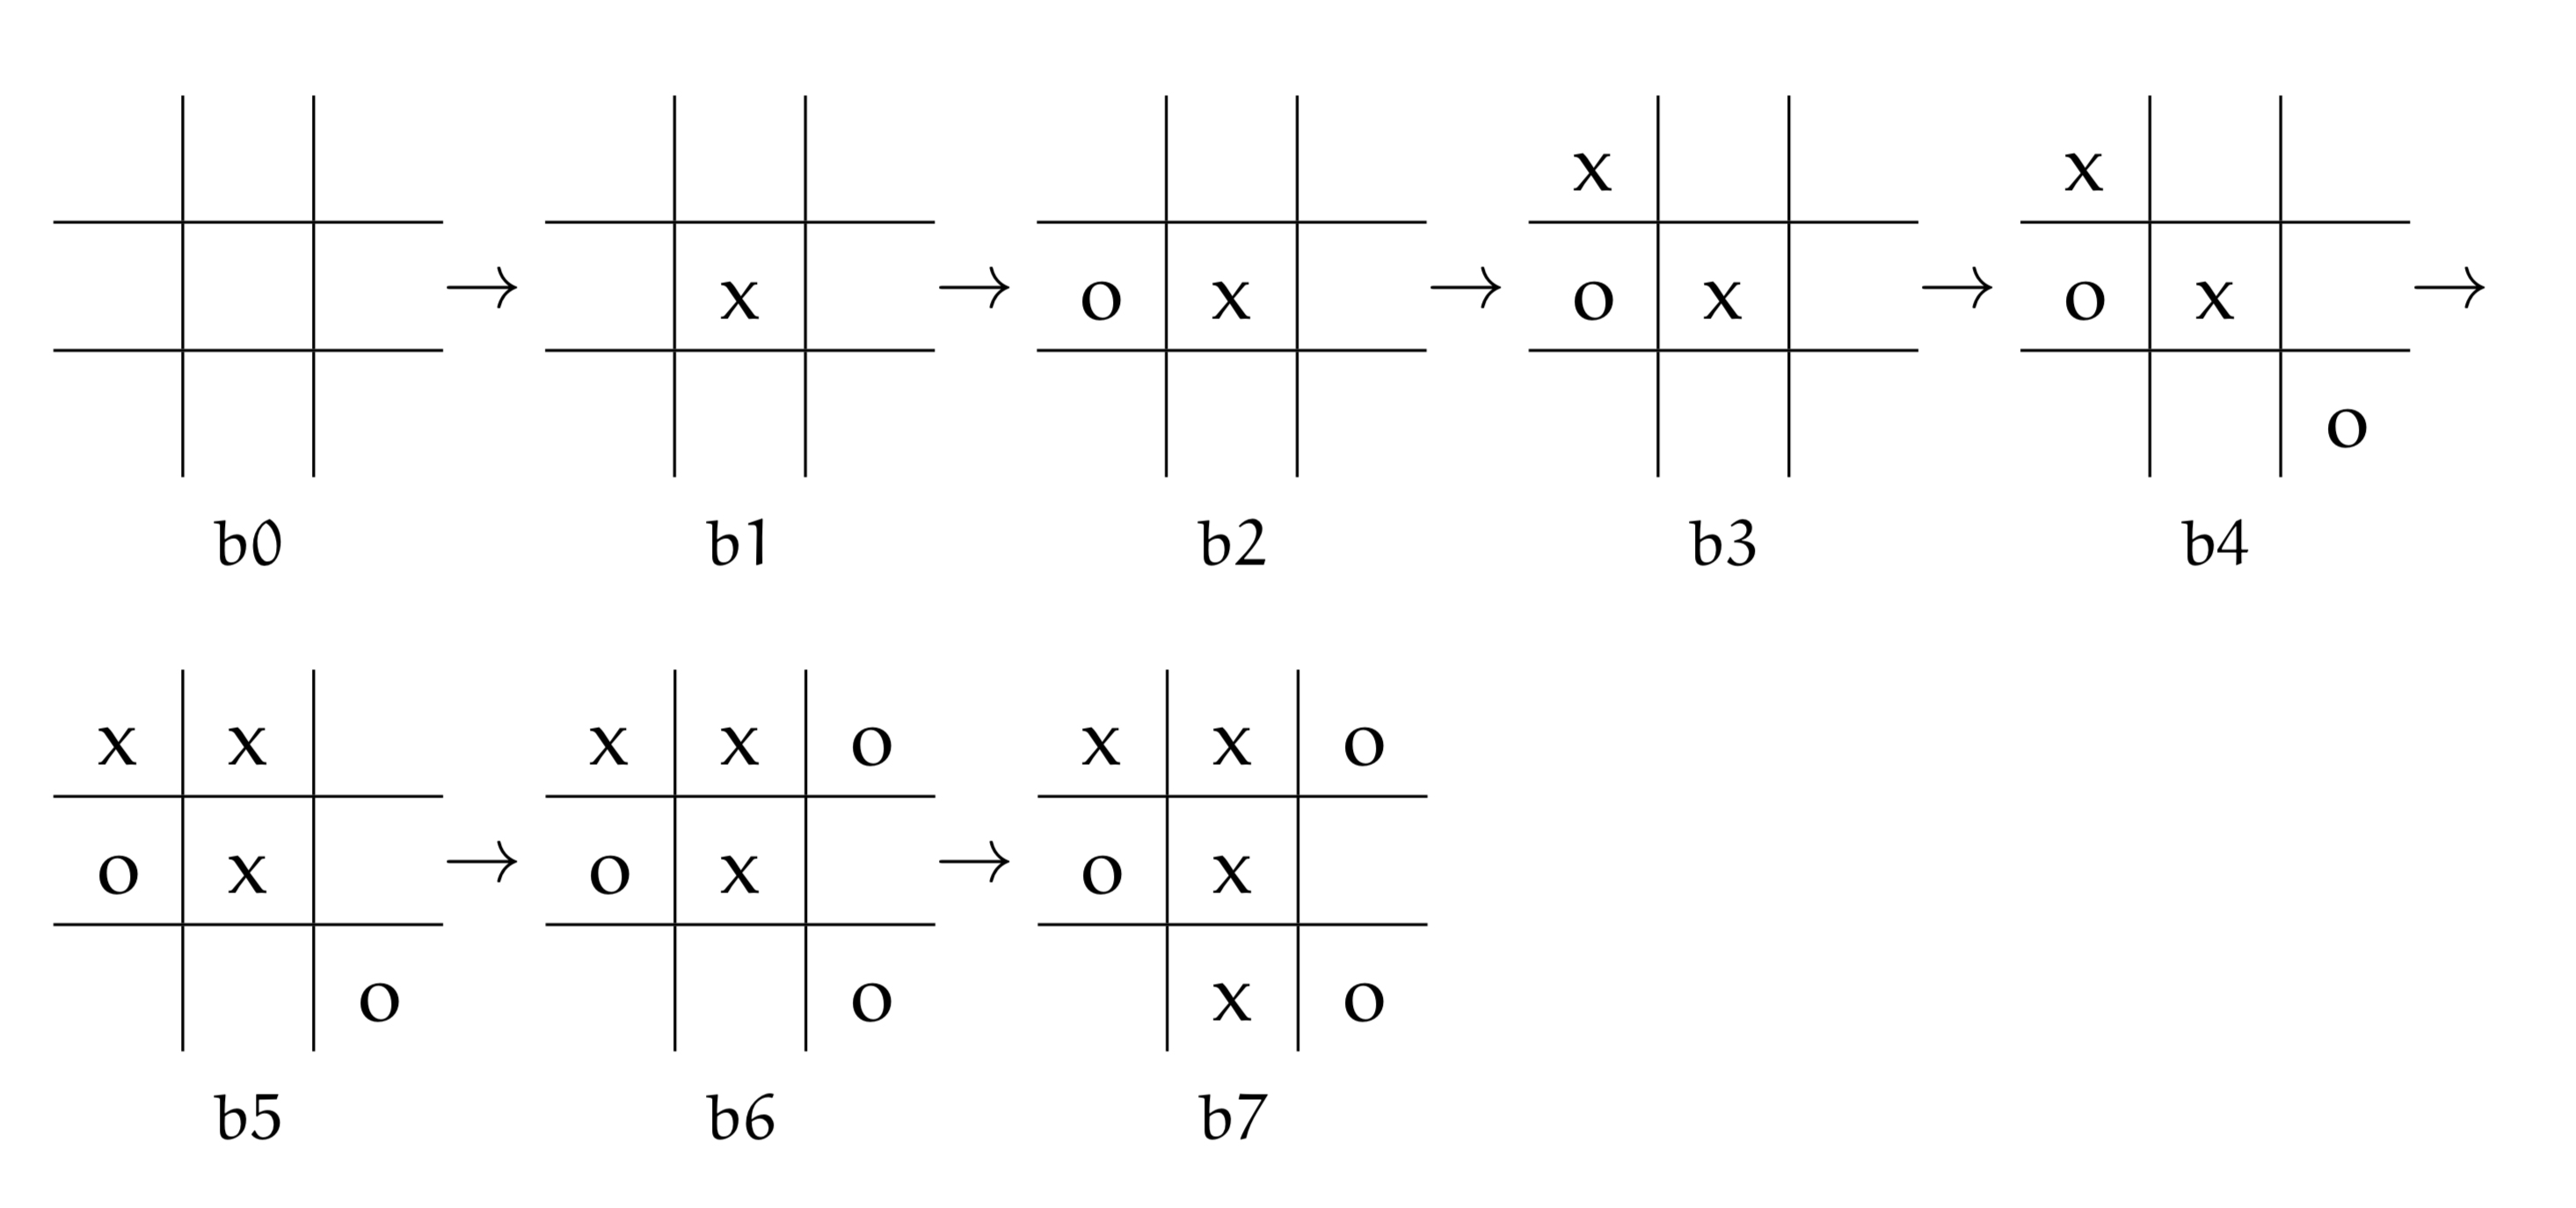
\includegraphics[width=\textwidth]{./images-defense/ttt-example.png}
\end{figure}
\end{frame}


\begin{frame}
\frametitle{Reinforcement learning: Results}
\begin{figure}
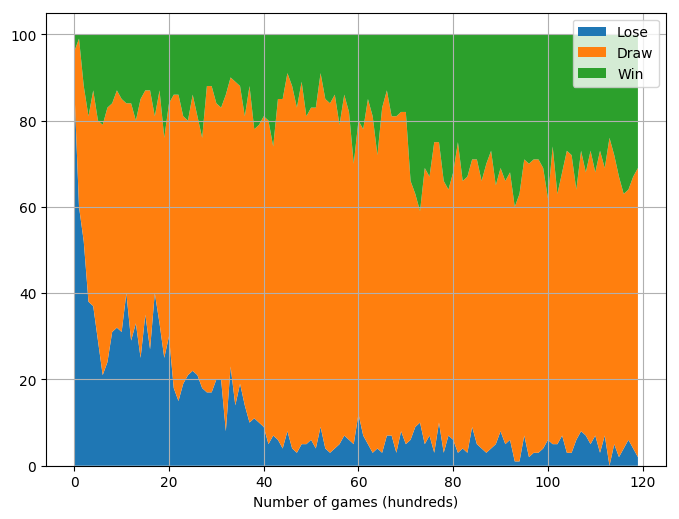
\includegraphics[width=0.7\textwidth]{./images02/ttt/results-smart.png}
\caption{Results playing against the smart player. Each cycle was made of 100 games for training, and then 100 games for measuring statistics.
\label{fig:ttt-results-smart}
}
\end{figure}
\end{frame}


%=============================================
%=============================================
%=============================================


\section{Diffusion and dismissal of innovation: forecasting the number of Facebook’s active users}
\begin{frame}
\sectionpage
\end{frame}


\begin{frame}
\frametitle{Diffusion and dismissal of innovation: forecasting the number of Facebook’s active users}

Based on the Bass Model, which is in the Top 10 Most Influential Papers in 50 years of the Management Science journal.

The Bass model assumes that there are two types of people: \textbf{the innovators} and \textbf{the imitators}---a simplification of Rogers' famous five classes (innovators, early adopters, early majority, late majority, and laggards).

The Bass model would be a good choice to forecast the total number of users. But most companies deem the total number of users as confidential, and \textbf{they only publish the number of active users}.

\end{frame}


\begin{frame}
\frametitle{The extended model}
\begin{align*}
\text{\textbf{Bass model:}} \\
\frac{f(t)}{1-F(t)} &= p + qF(t), F(0)=0 \\
\\
\text{\textbf{Proposed extension:}} \\
\frac{f(t)}{1-F(t)} &= p + qF(t) - wR(t), F(0)=0, R(0)=0
\end{align*}
\end{frame}


\begin{frame}
\frametitle{Contributions}
The main contributions are:
\begin{enumerate}[i]
\item Add a rejection parameter to the model
\item Estimate the parameters using only the number of active users \\(instead of the total number of users)
\item The possibility of reducing the number of active users \\(instead of only increasing)
\end{enumerate}
\end{frame}


\begin{frame}
\frametitle{Models of rejection}
\begin{align*}
	\text{Model 1: }& r(t) = \nu f(t) \\
    \\
	\text{Model 2: }& \frac{r(t)}{1-R(t)} = \nu f(t) \\
    \\
	\text{Model 3: }& r(t) = \nu [F(t) - R(t)] \\
    \\
	\text{Model 4: }& \frac{r(t)}{1-R(t)} = \nu [F(t) - R(t)]
\end{align*}
\end{frame}

\begin{frame}
\frametitle{Results: Model 2}
\begin{figure}
	\centering
	{\includegraphics*[scale=0.9,width=0.65\textwidth]{images03/fb-model2-1.eps}}
	\caption{Fit of Model 2 with Facebook's active users dataset.\label{fig:model2fit}
		{$mF(t)$ is the total users, $mR(t)$ is the inactive users, and $mA(t)$ is the active users. The unit of these functions are thousands of people. The parameters are $m=1,497.50$, $p=0.000331$, $q=0.100088$, $w=0.140595$, and $\nu=0.187188$. The goodness of fit are $R^2=99.84\%$ and BIC=10,566.52.}}
\end{figure}
\end{frame}


\begin{frame}
\frametitle{Results: Model 3}
\begin{figure}
	\centering
	{\includegraphics*[scale=0.9,width=0.65\textwidth]{images03/fb-model3-1.eps}}
	\caption{Fit of Model 3 with Facebook's active users dataset.\label{fig:model3fit}
		{$mF(t)$ is the total users, $mR(t)$ is the inactive users, and $mA(t)$ is the active users. The unit of these functions are thousands of people. The parameters are $m=1,967.64$, $p=0.000184$, $q=0.097867$, $w=0.330511$, and $\nu=0.006912$. The goodness of fit are $R^2=99.83\%$ and BIC=11,485.68}}
\end{figure}
\end{frame}


\begin{frame}
\frametitle{Results: Model 4}
\begin{figure}
	\centering
	{\includegraphics*[scale=0.9,width=0.65\textwidth]{images03/fb-model4-1.eps}}
	\caption{Fit of Model 4 with Facebook's active users dataset.\label{fig:model4fit}
		{$mF(t)$ is the total users, $mR(t)$ is the inactive users, and $mA(t)$ is the active users. The unit of these functions are thousands of people. The parameters are $m=1,854.85$, $p=0.000183$, $q=0.099738$, $w=0.334454$, and $\nu=0.007007$. The goodness of fit are $R^2=99.84\%$ and BIC=10,724.55}}
\end{figure}
\end{frame}


\begin{frame}
\titlepage
\end{frame}

\end{document}
